
\begin{refsection}
\startcontents[chapters]	
\chapter{Theory of Probability}\label{ch:theory-of-probability}
%\minitoc

\printcontents[chapters]{}{1}{}
\section{Sigma algebra}
\subsection{sigma algebra concepts}
\begin{definition}[$\sigma$ algebra]\index{$\sigma$-field}\index{$\sigma$-algebra}
Given a set $\Omega$, a $\sigma$-field, or $\sigma$-algebra is a collection $\mathcal{F}$ of subsets of $\Omega$, with the following properties:
\begin{enumerate}
\item $\emptyset \in \cF$
\item if $A \in \cF$, then $A^c \in \cF$
\item (countable union)if $A \in \cF$, then $\cup_{i=0}^{\infty}A_i \in \cF$
\end{enumerate}
\end{definition}

\begin{example}\hfill
\begin{enumerate}
\item The trivial $\sigma$-field $\cF = \{ \emptyset, \Omega \}$
\item The collection $\cF=\{\emptyset, A, A^c,\Omega \}$, where $A$ is a fixed subset of $\Omega$
\item The set of all the subsets of finite set $\Omega$.
\item For a finite sample space $\Omega$, the power set of $\Omega$ is the largest $\sigma$ field, $\{\emptyset,\Omega\}$ is the smallest $\sigma$ field.
\end{enumerate}
\end{example}


\begin{remark}
The pair $(X,\cF)$ is called \textbf{measurable space}, the members  $e\in \cF$ are called \textbf{measurable sets} or $\Sigma-$measurable sets.
\end{remark}



\begin{lemma}[intersection theorem] \label{theorem:sigmafieldintersect}\cite{dineen2013probability} 
If $\{\mathcal{F}_{\alpha}\}_{\alpha \in T}$ is a collection of $\sigma$ fields on $\Omega$, then $\cap_{\alpha \in T} \mathcal{F}_{\alpha}$ is $\sigma$ field on $\Omega$
\end{lemma}
\begin{proof}
We consider the special case $T=\{1,2\}$. Let $A = \mathcal{F}_1 \cap \mathcal{F}_2$. It is easy to see $\emptyset \in A$; since $A \in \cF_1 \cap \cF_2$, then $A \in \cF_1,A\in \cF_2$, then $A^c \in \cF_1, A^c \in \cF_2$, then $A^c\in \cF_1\cap \cF_2$; Similarly, we can prove the union property.
\end{proof}


\subsection{Generation of sigma algebra}

\begin{lemma}[Existence of smallest $\sigma$ field, $\sigma$ algebra generation]\label{ch:theory-of-probability:th:sigmafieldGeneration}\index{$\sigma$ field generation}
 If $\mathcal{A}$ is a collection of subsets of $\Omega$, then there exist a unique smallest $\sigma$ field on $\Omega$, containing $\mathcal{A}$, which is contained by all the $\sigma$ fields that contains $\mathcal{A}$. We denote this by $\cF(\mathcal{A})$, and called the $\sigma$ field generated by $\mathcal{A}$.\cite{dineen2013probability}
\end{lemma}
\begin{proof}
Consider $\mathcal{B}$ as the set of all $\sigma$ fields that contains $\mathcal{A}$. The intersections of all these sets will lead to $\cF(\mathcal{A})$ due to theorem \ref{theorem:sigmafieldintersect}.
\end{proof}

\begin{definition}[sigma algebra generated by an event]
	Let $A$ be a subset of a sample space $\Omega$. The sigma algebra generated by $A$, denoted by $\sigma(A)$, is a set given by
	$$\sigma(A) = \{\emptyset, \Omega, A, A^c\}.$$	
\end{definition}

\begin{remark}[sigma algebra generated by random variable and stochastic process]
The generation of sigma algebra by random variables and stochastic processes are discussed in \autoref{ch:theory-of-probability:def:sigmaAlgebraGeneratedByRandomVariable}\autoref{ch:theory-of-stochastic-process:def:NaturalFiltrationGeneratedByStochasticProcesses}.	
\end{remark}



\begin{corollary}
(Properties of generated $\sigma$ algebra) If $\cA,\cA_1$ and $\cA_2$ are subsets of $2^\Omega$, then we have \cite{dineen2013probability}
\begin{itemize}
    \item If $\cA_1 \subset \cA_2$, then $\cF(\cA_1) \subset \cF(\cA_2)$
    \item If $\cA$ is a $\sigma$ field, then $\cF(\cA) = \cA$
    \item If $\cF(\cF(\cA)) = \cF(\cA)$
\end{itemize}
\end{corollary}


\subsection{Partition of sample space}
\begin{definition}
A collection of subsets of $\Omega$, $\{\cA_i \}_{i\in I}$ ($I$ can have size of uncountable infinite)is called a partition of $\Omega$ if
$$\cA_i \cap \cA_j = \emptyset, ~\text{if}~ i\neq j $$
and $$\cup A_i = \Omega.$$
\end{definition}

\begin{lemma}\cite{dineen2013probability}
If $\mathcal{P}=\{ A_i \}_{i\in 1}^\infty$ is a countable partition of $\Omega$, then the $\sigma$ field generated from $\mathcal{P}$, $\cF(\mathcal{P})$, consists of all sets of the form $\cup_{n\in M} A_n$ where $M$ ranges over all subsets of $\mathbb{N}$.
\end{lemma}

\begin{lemma}
Let $\cP_1,\cP_2$ be the partitions of the same sample space $\Omega$. If $\cP_2$ is obtained by subdividing sets in $\cP_1$ (i.e. $\cP_2$ is finer), then we have
$$\cF(\cP_1)\subseteq \cF(\cP_2) \Leftrightarrow \cP_1 \subseteq \cP_2$$
\end{lemma}

\subsection{Filtration \& information}


\begin{definition}[filtration]\index{filtration}
Let $(\Omega,\mathcal{F})$ denote a measurable space.
\begin{itemize}
    \item A \textbf{continuous filtration} is defined as:
A family of $\sigma$ algebras $\{\mathcal{F}_t|t>=0\}$ where 
$$ \mathcal{F}_s \subseteq \mathcal{F}_t \subseteq \mathcal{F}, 0 \leq s \leq t$$
\item A \textbf{discrete filtration} on $(\Omega,\cF)$ is an increasing sequence of $\sigma$ fields $\{\cF_n\}$ such that:
$$\cF_1 \subseteq \cF_2 ... \subseteq \cF$$
\end{itemize}
Note that as the time progresses, the finer the $\sigma$ algebra will be. We call $\cF_n$ the history up to time $n$.
\end{definition}


\begin{remark}
	Note that usually not all the subsets of $X$ can be defined a measure with above properties. For example, all irrational numbers in the real line, the root to polynomial equation, are not measurable sets.\cite{rosenthal2006first} 
\end{remark}

\begin{remark}[filtration and information]\hfill
\begin{itemize}
	\item Let $\cF_1, \cF_2$ be two $\sigma$ field on $\Omega$, then $\cF_1 \subseteq \cF_2$ mean $\cF_2$ contains more information than $\cF_1$; For any $A$ is measurable with respect to $\cF_1$ then $A$ is measurable with respect to $\cF_2$. That is, if $A\subset \cF_1$ then $A\subset \cF_2$.
\end{itemize}		
\end{remark}

\begin{example}
	For example, in a die toss example, $\cF_1$ is generated by the events of odd number or even number, while $\cF_2$ is generated by the event of all possible outcomes. Then, we have $\cF_1 \subset \cF_2$,i.e., knowing the probability measure on $\cF_2$ will enable us to calculate the probability measure on $\cF_1$.\cite{dineen2013probability} 
	
	Now consider a series of experiment: Let $\Omega$ denote the set of all outcomes resulting from tossing a coin three times, the $\Omega = \{(H,H,H),(T,H,H)...,(T,T,T)\}$. Let $\cF_i$ denote the events that have been determined by the end of the $i$ toss. Then $\cF_1=\cF(\{(H,\cdot,\cdot),(T,\cdot,\cdot)\})$, where $\cdot$ represent it will range over $H,T$,i.e., $\cF_1$ is generated from a partition of 2. Since we have more information later, we have
	$$\cF_1 \subset \cF_2 \subset \cF_3$$
	Note that if $\cF_2$ represents events determined by the $i$ toss instead of tosses upto $i$, the above will not hold.
\end{example}


\subsection{Borel $\sigma$ algebra}
\begin{definition}\index{Borel set}\index{Borel algebra}\cite{wiki:Borelset}
A Borel set  is any set in a topological space that can be formed from open sets (or, equivalently, from closed sets) through the operations of countable union, countable intersection, and relative complement. For a topological space $X$, the collection of all Borel sets on $X$ forms a $\sigma$-algebra, known as the Borel $\sigma$-algebra. The Borel $\sigma$ algebra on $X$ is the smallest $\sigma$-algebra generated by open sets.
\end{definition}

\begin{remark}
Note that the elements like low-dimensional manifold $S\subset \R^m, m<n$ in $\R^n$ will not be in the $\mathcal{B}(\R^n)$, i.e., they cannot be obtained from open set operation defined above. 
\end{remark}


\begin{note}[open interval close interval conversion]
Using countable union and intersection properties, we can convert between open interval and close intervals, for example
\begin{itemize}
	\item $(a,b)=\cup_{n=1}^{\infty}[a+1/n,b-1/n]$
	\item $[a,b]=\cap_{n=1}^{\infty}(a-1/n,b]$
	\item $(a,\infty) = \cup_{n=1}^{\infty}[a,a+n]$
	\item singleton: $\{a\} = [a,a]$
\end{itemize}	
\end{note}



\subsection{Measurable set and measurable space}\index{measurable set}\index{measurable space}\index{measure}


\begin{definition}
Given a set $X$ with its $\sigma$ field $\Sigma$, a function $\mu: \Sigma \rightarrow \R$ is called a \textbf{measure} if it satisfies: \cite{wiki:measure}:
\begin{itemize}
    \item Non-negativity: For all $E \in \Sigma$, $\mu(E)>=0$
    \item $\mu(\emptyset) = 0$
    \item Countable additivity: For all countable collections $\{E_i\}$ of pairwise disjoint sets in $\Sigma$:
    $$\mu(\cup_{i=1} E_i) = \sum_{i=1} \mu(E_i)$$
\end{itemize}

The pair $(X,\Sigma)$ is called \textbf{measurable space}, the members  $e\in \Sigma$ are called \textbf{measurable sets} or $\Sigma-$measurable sets. A triple $(X,\Sigma,\mu)$ is called measure space. A \textbf{probability measure} is a measure with total measure one $\mu(X) = 1$. A probability space (i.e. a triple) is a measure space with a probability measure.\cite{dineen2013probability}
\end{definition}

\begin{remark}
A \textbf{measure} on a set is a systematic way to assign a number of each suitable subset of set, as a generalization of the concepts of length, area, and volume. 	
\end{remark}


\begin{definition}[measurable function]\index{measurable function}
Let $(\Omega,\cF)$ be a measurable space. A function $f:\Omega \to \R$ is said to be $\cF$-measurable if $f^{-1}(B)\in \cF,B\in \mathcal{B}(R)$.
\end{definition}

\begin{theorem}[measurable function with coarse sigma field]
Let $\cF$ generated by a finite partitions $B_1,B_2,...,B_m$ of $\Omega$; let function $f:\Omega\to \R$ be $\cF$\textbf{-measurable}. Then $f$ takes constant value on each element of $B_i,1\leq i \leq m$. 
\end{theorem}
\begin{proof}
Suppose $f$ can take different values, say $a_1,a_2$, then the inverse image of the interval $[a_1,0.5(a_1+a_2)]$ is not a subset of $\cF$ (note that $\cF$ can only contain $\emptyset$ plus subsets due to unions of partition subset. See previous sections on partition of sample space), which contradicts the fact of $f$ is measurable. 
\end{proof}

\begin{figure}[H]
	\centering
	\begin{subfigure}[b]{0.4\textwidth}
		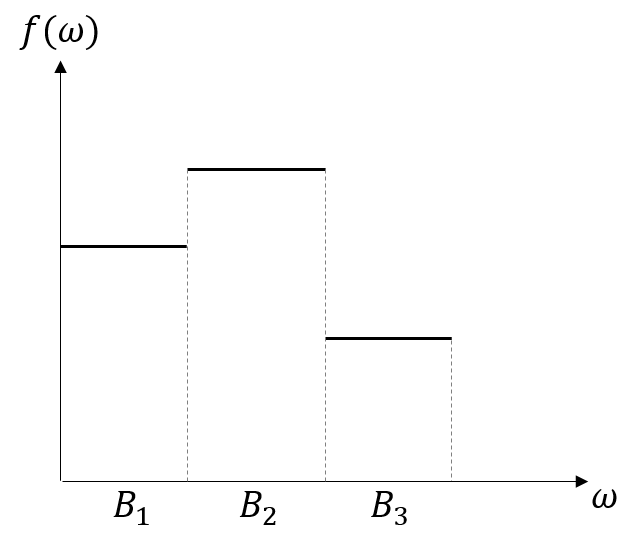
\includegraphics[width=\textwidth]{figures/mathFundamentals/measurableFunctionDemo1}
		\caption{A mesurable function measurable with respect to the $\sigma$ algebra generated by partition $B_1,B_2,B_3$.}
	\end{subfigure}\quad
	\begin{subfigure}[b]{0.4\textwidth}
		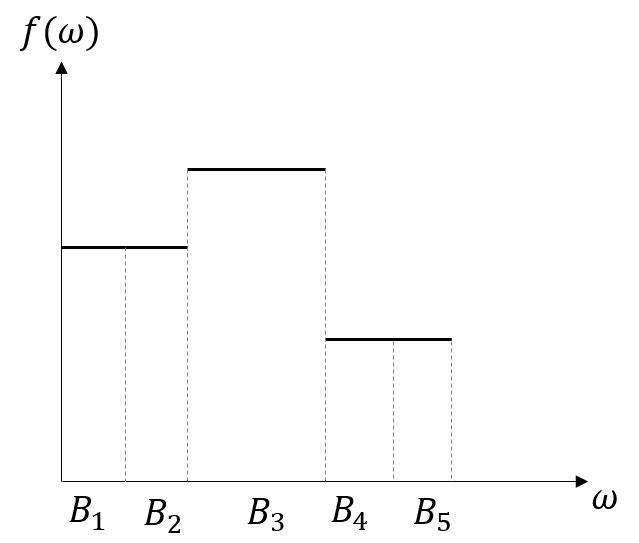
\includegraphics[width=\textwidth]{figures/mathFundamentals/measurableFunctionDemo2}
		\caption{A mesurable function measurable with respect to the $\sigma$ algebra generated by partition $B_1,B_2,B_3,B_4,B_5$.}
	\end{subfigure}\quad
	\begin{subfigure}[b]{0.4\textwidth}
		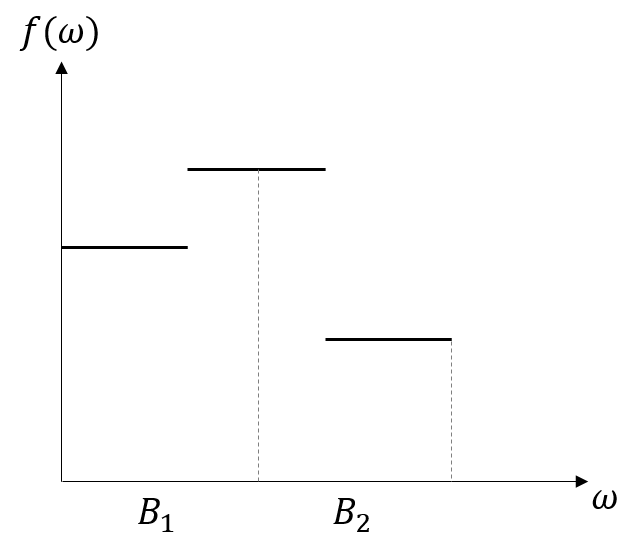
\includegraphics[width=\textwidth]{figures/mathFundamentals/measurableFunctionDemo3}
		\caption{A function not measurable with respect to the $\sigma$ algebra generated by partition $B_1,B_2$.}
	\end{subfigure}\quad
	\caption{An illustration of measurable functions.}
\end{figure}

\begin{note}[measurable functions vs. ordinary functions]\hfill
\begin{itemize}
	\item Ordinary functions from set $A$ to set $B$ simply establish a relationship between elements in $A$ and elements in $B$. A measurable function from set $A$ to set $B$ also establish a relationship between elements in $A$ and elements in $B$, however, under the constraint of measurability of $\sigma$ fields.
	\item The level of coarseness constrain the number of values a measurable function can take. For a trivial $\cF$, its measurable function can only take one value.
	\item For random variables, they are required to be measurable functions.
\end{itemize}	
\end{note}





\section{Probability space}\index{probability space}

\subsection{Event, sample point and sample space}\index{event}\index{sample space}
\begin{definition}[event,sample point and sample space]\index{event}
	Consider a random experiment. The collection of all outcomes is the sample space $\Omega$. 
	Given a sample space $\Omega$ with its $\sigma$ field $\mathcal{F}$, an event is simply an element in  $\mathcal{F}$.	
\end{definition}

\begin{remark}[interpretation]\hfill
	\begin{itemize}
		\item The results of experiments or observations are called events. For example, the result of a measurement will be called an event. We shall distinguish between \emph{compound}(or decomposable) and \emph{simple}(or indecomposable) \emph{events}. For example, saying that a throw with two dice resulted in "sum six" amounts to saying that it resulted in (1,5) or (2,4) ..., which can be decomposes to five simple events. 
		\item The simple events will be called sample points. Every dis-decomposable result of the experiment is represented by one and only one, sample point. The aggregate of \emph{all} sample points will be called sample space. 
	\end{itemize}	
\end{remark}




\subsection{Probability space}
\begin{definition}[probability space]\cite{rosenthal2006first}\label{ch:theory-of-probability:def:ProbabilitySpace}
A probabilistic model is defined formally by a triple $(\Omega, \mathcal{F}, P)$, called a probability space, where
\begin{enumerate}
\item $\Omega$ is the sample space, the set of possible outcomes of the experiment
\item $\mathcal{F}$ is a $\sigma$-field, a collection of subsets of $\Omega$, containing $\Omega$ itself and the empty set $\emptyset$, and closed under the formation of complements, countable unions, and countable intersections
\item $P$ is a \textbf{probability measure }defined on  $\sigma$-field $\mathcal{F}$, and has the property of: 
\begin{itemize}
\item $P(A)\geq 0, \forall A\in \cF$
\item if $A_1,A_2,... \in \cF$ are \textbf{disjoints} subsets of $\Omega$, we have \textbf{countable additivity} as:
$P(A_1\cup A_2 \cup A_3 ...) = P(A_1) + P(A_2) + P(A_3) + ...$
\item $P({\Omega}) = 1$.
\end{itemize}
\end{enumerate}
\end{definition}


\begin{remark}[interpretation]\hfill
\begin{itemize}
	\item Note that the $\sigma$-algebra is the collections of \emph{measurable sets}. These are the subsets $A \subseteq \Omega$ where $P(A)$ is defined. In general, $\sigma$-field might not contain \emph{all} subsets of $\Omega$(For example, let $\Omega$ be a interval on the real line, then the set of all rational number in the interval is not in $\sigma$-field)
	\item \textbf{Note that we cannot extend to \emph{uncountable unions};} in this case, $\mathbb{F}$ would contain every subset $A$, since every subset can be written as $A = \cup_{x\in A} \{x\} $ and since the singleton sets $\{x\}$ are all in $\mathbb{F}$.
\end{itemize}
\end{remark}


\begin{definition}[discrete probability space]
A discrete probability space is a triplet $(\Omega, \mathbb{F},\mathbb{P})$ such that
\begin{enumerate}
\item the sample space is finite or countable
\item the $\sigma$-field is the set of all subsets of $\Omega$
\item the probability measure (a function) assigns a number in the set [0,1] to every pairwise disjoint subset of $A\subseteq\Omega$, given as $$\mathbb{P}(A)=\sum_{\omega\in A} \mathbb{P}(\{\omega\})$$  and $$\sum_{\omega \in \Omega} \mathbb{P}(\{\omega\}) = 1$$
\end{enumerate}
\end{definition}

\begin{example}[Infinite coin toss process(infinite Bernoulli experiments)]\cite[4]{shreve2004stochastic2}\hfill
\begin{itemize}
	\item Consider the probability space for tossing a coin infinitely many time. We can define the sample space as $\Omega_\infty = \text{the set of infinite sequences of Hs and Ts}$. A generic element of $\Omega_\infty$ will be denoted as $\omega=\omega_1\omega_2....$, where $\omega_n$ indicates the result of the $n$th coin toss $\omega_n = H ~or~ T$.
	\item Example subsets in $\Omega$ are
	\begin{itemize}
		\item $A_H$: the set of all sequences beginning with $H$. $A_H = \{\omega: \omega_1= H\}$.
		\item $A_T$: the set of all sequences beginning with $H$. $A_T = \{\omega: \omega_1= H\}$.
		\item $A_{HT}$: the set of all sequences beginning with $HT$. $A_{HT} = \{\omega: \omega_1= H,\omega_1= T\}$.
		\item $A_{TH}$: the set of all sequences beginning with $TH$. $A_{TH} = \{\omega: \omega_1= T,\omega_2=H\}$.
	\end{itemize}
	\item Possible $\sigma$ algebra includes:
	\begin{itemize}
		\item $\cF_0 = \{0,\Omega_\infty\}$.
		\item $\cF_1 = \{0,\Omega_\infty, A_H,A_T\}$.
		\item 
		\begin{align*}
		\cF_2 &= \\
		&0,\Omega_\infty, A_H,A_T, A_{HH},A_{HT},A_{TH},A_{TT},A_{HH}^C,A_{HT}^C,A_{TH}^C,A_{TT}^C, \\
		&A_{HH}\cup A_{TH},A_{HH}\cup A_{TT},A_{HT}\cup A_{TH},A_{HT}\cup A_{TT} 
		\end{align*}
	
	\end{itemize}
\end{itemize}	





\end{example}




\subsection{Properties of probability measure}

\begin{lemma}[basic properties of probability measure]\cite[11]{hoggintroduction}
\begin{itemize}
	\item $P({\emptyset}) = 0$.
	\item (finite additivity)if $A_1,A_2,...,A_n \in \cF$ are \textbf{disjoints} subsets of $\Omega$, we have:
	$P(A_1\cup A_2 ... \cup A_n) = P(A_1) + P(A_2) + ... + P(A_n).$
	\item For each $A\in \cF$, $P(A^C) = 1 - P(A)$, where $A^C$ is the complement of $A$ with respect to $\Omega$.
	\item If $A_1,A_2 \in \cF$ and $A_1\subset A_2$, then $P(A_1)\leq P(A_2)$.
	\item For $B\subset A$, $P(A-B) = P(A) - P(B)$.
\end{itemize}	
\end{lemma}
\begin{proof}
(1) Directly from 
$$P(\cup \emptyset) = P(\emptyset) = \sum P(\emptyset)$$
and $P(\emptyset) \geq 0$, we have $P(\emptyset) = 0$.
(2) Set $A_{n+1},A_{n+2},... = \emptyset$ and use (1). (3) from (2). (4) note that $A_2 = A_1 + (A_2-A_1)$ and $P(A_2-A_1)\geq 0$.
(5) Note that $(A-B)\cup B = A$ such that
$$P(B) + P(A-B) = P(A).$$
\end{proof}





\begin{lemma}[union bound]\index{union bound}
For any sequence $A_1,A_2,... \in \mathcal{F}$
$P(A_1\cup A_2 \cup A_3 \cup ...) \leq P(A_1) + P(A_2) + ... $
\end{lemma}
\begin{proof}
 Based on countable additivity of probability function, we have:
\begin{align*}
P(A_1\cup A_2 \cup A_3 \cup ...) = P(A_1 \cup (A_2\backslash A_1) \cup (A_3\backslash A_2 \backslash A_1)...)\\
= P(A_1) + P(A_2 \backslash A_1) ... <= P(A_1) + P(A_2) + ...    
\end{align*}
\end{proof}



\subsection{Conditional probability}
\subsubsection{Basics}


\begin{remark}[general remarks]\hfill
	\begin{itemize}
		\item In some random experiments, we are interested only in those outcomes that are elements of a subset $C_1$ of the sample space $\Omega$. Then given the probability space $(\Omega,\mathcal{F},P)$, and  $C_1,C_2 \in \mathcal{F}$, the conditional probability of the event $C_2$, given $C_1$ is defined as 
		$$P(C_2 | C_1) = \frac{P(C_1\cap C_2)}{P(C_1)}.$$
		\item Note that usually, for two events $C_1,C_2$ both occur, we can define an new event $C_3 = C_1 \cap C_2$, then we write $P(C_1,C_2) = P(C_3) = P(C_1\cap C_2)$. $P(C_1\cap C_2)$ is quite formal since it is based on set theory.
	\end{itemize}	
\end{remark}

\begin{definition}[conditional probability measure]
	Given a probability space $(\Omega, \cF, P)$ and an event $A\in \cF, P(A)\neq 0$, we can define a conditional probability measure
	$$P_A(B) \triangleq P(B|A) = \frac{P(A\cap B)}{P(A)}.$$		
\end{definition}

\begin{lemma}[basic properties of conditional probability measure]\cite{hoggintroduction}
	Consider the conditional probability measure conditioned on event $A$. We have	
	\begin{itemize}
		\item $P(B|A) \geq 0, \forall B\in \cF$.
		\item $P(B|A) = 0, \forall B\in \cF, A\cap B$.
		\item $P(A|A) = 1$.
		\item $P(\cup_{j=1}^\infty B_i|A) = \sum_{j=1}^\infty P(B_i|A),$ provided that $B_1,B_2,...\in \cF$ are mutually exclusive event.
		
		\item $\sum_{i=1}^\infty P(C_i|A) = 1$, where $C_1,C_2,... \in \cF$ are the partition of $\Omega$.
	\end{itemize}	
\end{lemma}
\begin{proof}
	(4)Use countable additivity property of the definition of probability space
	\autoref{ch:theory-of-probability:def:ProbabilitySpace}, we have
	$$P(\cup_{j=1}^\infty B_i|A) = \frac{P(\cup_{j=1}^\infty  B_i\cap A)}{P(A)} = \sum_{j=1}^\infty \frac{P(B_i\cap A)}{P(A)} = \sum_{j=1}^\infty P(B_i|A).$$
	(5) Note that $\cup_{i=1}^\infty (C_i\cap A) = A$.
\end{proof}

\begin{lemma}[Law of total probability]\index{Law of total probability}\label{ch:theory-of-probability:th:lawoftotalprobability}
	Given a set of subsets $C_1,C_2,...,C_k$, which are mutual disjoint and partition the sample space $\Omega$, then we have 
	$$P(C) = P(C\cap C_1) + P(C\cap C_2)... + P(C\cap C_k) = \sum_{i=1}^k P(C_i)P(C|C_i)$$
\end{lemma}
\begin{proof}
	Note that we have $P(C\cap C_i) = P(C_i)P(C|C_i)$, then we get the law of total probability as:
	$$P(C) = P(C_1)P(C|C_1) + P(C_2)P(C|C_2)+.. +P(C_k)P(C|C_k) = \sum_{i=1}^k P(C_i)P(C|C_i)$$		
\end{proof}

\begin{theorem}[Bayes' theorem]\index{Bayes' theorem}
	From the definition of the conditional probability, we have Bayes' theorem as: 
	$$P(C_j|C) = \frac{P(C\cap C_j)}{P(C)} = \frac{P(C_i)P(C|C_i)}{\sum_{i=1}^k P(C_i)P(C|C_i)}$$	
\end{theorem}
\begin{proof}
	The law of total probability has been in the denominator.
\end{proof}

\begin{theorem}[Conditional Bayes' theorem]\index{conditional Bayes' theorem}
	From the definition of the conditional probability, we have Bayes' theorem as: 
	$$P(C_j|C) = \frac{P(C\cap C_j)}{P(C)} = \frac{P(C_i)P(C|C_i)}{\sum_{i=1}^k P(C_i)P(C|C_i)}$$	
\end{theorem}
\begin{proof}
	The law of total probability has been in the denominator.
\end{proof}

\subsubsection{Independence of events and sigma algebra}
\begin{definition}[independence of event]
	Given the probability space $(\Omega,\mathcal{F},P)$, and  $C_1,C_2 \in \mathcal{F}$, then we say $C_1$ and $C_2$ are independent if
	$$P(C_1\cap C_2) = P(C_1)P(C_2).$$	
\end{definition}

\begin{definition}[independence of $\sigma$ algebras]
Given the probability space $(\Omega,\mathcal{F},P)$, and  $\cF_1,\cF_2 \subset \cF$, then we say $\cF_1$ and $\cF_2$ are independent if
$$P(A_1\cap A_2) = P(A_1)P(A_2),\forall A_1\in \cF_1,A_2\in \cF_2.$$	
\end{definition}

\begin{remark}
	Note that this is mathematical equivalent definition, which does not reveal the nature of independence in terms of set relationship. \textbf{The nature is that if two events are independent, then the occurrence of one event will not change our brief on the occurrence of the other event.}
\end{remark}

\begin{example}
	Consider the sample space of a random experiment is given as $\{(0,0),(0,1),(1,0),(1,1)\}$, with its $\sigma$ field consists of all its subsets, and we define event $C_1=\{(0,0),(0,1)\}$, and $C_2\{(0,1)\}$. So the occurrence of $C_1$ will change the our brief of $C_2$ from 1/4 to 1/2. Therefore, $C_1$ and $C_2$ are not independent to each other.  Also, consider $C_3 = C_1^c$, then the occurrence of $C_1$ change our brief of $C_1^c$ to 0. If $C_4 = \Omega$, then the occurrence of $C_4$ will not change, and thus $C_4$ is always independent of other events. In summary, \textbf{independence between events is far more complicated than the simple set relations between events} 	
\end{example}

\begin{remark}
	Here is an non-trivial example of independence. Consider the sample space as the product of two coin toss sample space, the event that the first toss get 1 is $\{(1,0),(1,1)\}$, which is independent of the other event that the second toss get 1(i.e. $\{(0,1),(1,1)\}$). The two events have finite intersections, but they are independent. Therefore, it seems that simply considering the set relationships between events can not yield complete information of independence. The nature of the random experiment, i.e., the probability measure, dictates the Independence. The intuition way to judge independence will be whether the occurrence of one events provides useful information, i.e., changes our brief, for the occurrence of the other event.	
\end{remark}


\begin{lemma}
	If $C_1,C_2$ are independent, then $C_1$ and $C_2^c$,$C_1^c$ and $C_2$, $C_1^c$ and $C_2^c$ are independent. 	
\end{lemma}

\begin{lemma}\cite{dineen2013probability}\hfill
	\begin{itemize} 
		\item If $P(A) > 0 $, then $A$ and $B$ are independent if and only if $P(B|A) = P(B)$
		\item If $A$ and $B$ are independent, then $A$ and $B^C$ are independent.
		\item If $P(A)=0$ or 1, then for any $B\in \cF,B\neq A$, $A$ and $B$ are independent.    
	\end{itemize}
\end{lemma}
\begin{proof}
	(1) Suppose $A$ and $B$ are independent, then
	$$P(A\cap B) = P(A)P(B) = P(A)P(B|A)\implies P(B|A) = P(B).$$
	(2) $$P(A\cap B^C) = P(A \cap (\Omega - B)) = P(A\cap \Omega) - P(A\cap B) = P(A) - P(A)P(B) = P(A)P(B^C).$$
	(3) If $A = \Omega$ such that $P(A) = 1$,then
	$$P(A\cap B) = P(B) = P(A)P(B).$$	
	If $A = \emptyset$ such that $P(A) = 0$,then
	$$P(A\cap B) = P(A) = 0 = P(A)P(B).$$
\end{proof}




\section{Measurable map and random variable}\index{mensurable map}\index{random variable}
\subsection{Random variable}
\begin{definition}[measurable map]\cite{fries2007mathematical}
Let $(\Omega,\mathcal{F})$ and $(S,\mathcal{S})$ be two measurable space.
 A map $T:\Omega \rightarrow S$ is called $(\mathcal{F},\mathcal{S})$\textbf{-measurable map} if
    $$T^{-1}(A)\in \mathcal{F}, \forall A\in \mathcal{S}$$We can also write it as $$T:(\Omega,\mathcal{F})\rightarrow (S,\mathcal{S}).$$
\end{definition}



\begin{definition}[random variables]
Let $(\Omega,\mathcal{F})$ and $(S,\mathcal{S})$ be two measurable space.	
    A measurable map $X:(\Omega,\mathcal{F})\rightarrow (S,\mathcal{S})$ is also called a \textbf{random variable} if $S=\R^n,\mathcal{S}=\mathcal{B}(\R^n)$; $X$ is called a \textbf{n-dimensional real-valued random vector}if $S=\R,\mathcal{S}=\mathcal{B}(\R)$.	
\end{definition}

\begin{remark}[interpretation]\hfill
\begin{itemize}
	\item Note that the measurability property of the map enables us to measure some suitable subsets of the image $S$ of random variable $X$ \emph{consistently} with the measure in the origin measurable space $(\Omega,\mathcal{F})$.
\end{itemize}	
\end{remark}


\begin{lemma}[basic properties of measurable map]\label{ch:theory-of-probability:th:BasicPropertiesOfMeasurableMap}
Let $(\Omega,\mathcal{F})$ and $(S,\mathcal{S})$ be two measurable space. Let a map $T:\Omega \rightarrow S$ be a measurable map. Then we have:
\begin{itemize}
	\item For any two disjoint sets $S_1,S_2 \in \mathcal{S}$, $T^{-1}(S_1)$ and $T^{-1}(S_2)$ are disjoint.
	\item $T^{-1}(S) = \Omega$.
	\item (measurable composition preserves measurability)Let $G$ be a measurable map from $(S,\cS)$ to $(S,\cS)$. Then $G\circ T: \Omega \to S$ is a measurable map.
\end{itemize}
\end{lemma}
\begin{proof}
(1) Suppose their inverse image intersection $M$ is nonempty, then $T(m),m\in M$ will map a single element to two different elements in $S$, which violates the definitions of mapping.
(2) Suppose $T^{-1}(S) = \Omega_1 \subset \Omega$ and $\Omega_1 \neq  \Omega$, then $T(\Omega - \Omega_1) = \emptyset$(otherwise $T$ will map a single element to two different elements). Therefore $T^{-1}(S\cup \emptyset) = T^{-1}(S) = \Omega$. (3) Note that $(G\circ T)^{-1}(B) = T^{-1}\circ G^{-1} (B) = T^{-1}( G^{-1} (B)) $
Because $G$ is measurable map, $G^{-1} (B) \in \cS$. Because $T$ is measurable map, $T^{-1}( G^{-1} (B)) \in \cF$. Therefore, $G\circ T$ is a measurable from $\Omega$ to $S$. 
\end{proof}

\begin{lemma}[basic measurability properties of random variables]\label{ch:theory-of-probability:th:BasicMeasurabilityPropertyRandomVariables}
Let $(\Omega,\mathcal{F})$ and $(\R,\mathcal{B})$ be two measurable space. Let $X:\Omega \rightarrow \R$ be a random variable. Then we have:
\begin{itemize}
	\item  (measurable composition preserves measurability)Let $f$ be a measurable map from $(S,\cS)$ to $(S,\cS)$. Then $f(X): \Omega \to \R$ is a measurable map.
	\item Let $Y$ be another random variable from $(\Omega,\cF)$ to $(R,\cB)$. Then $\alpha X + \beta Y: \Omega \to \R, \alpha,\beta\in \R$ is also a measurable map.
	\item Let $Y$ be another random variable from $(\Omega,\cF)$ to $(R,\cB)$. Then $XY: \Omega \to \R$ is also a measurable map.
	\item Let $Y, Y\neq 0$ be another random variable from $(\Omega,\cF)$ to $(R,\cB)$. Then $1/Y: \Omega \to \R$ is also a measurable map.
\end{itemize}	
\end{lemma}
\begin{proof}
(1) Use the composition property of measurable map(\autoref{ch:theory-of-probability:th:BasicPropertiesOfMeasurableMap}).	(2)(3)(4) use \autoref{ch:calculus:th:AlgebraicPropertiesBorelMeasurableFunctions}.
\end{proof}

\begin{remark}[implications]
This theorem provides the foundation of when $X$ and $Y$ are random variables, usually, $f(X), X+Y, XY, X/Y,...$ are also random variables. 	
\end{remark}

\subsection{Image measure}
\begin{definition}[image measure]\cite{fries2007mathematical}
Let $X:(\Omega,\mathcal{F})\rightarrow (S,\mathcal{S})$ denote a random variable and $P$ a measure on the measurable space $(\Omega,\mathcal{F})$. Then
$$P_{X}(A):=P(X^{-1}(A)),\forall A \in \mathcal{S}$$
defines a probability measure on $(S,\mathcal{S})$, which we call the image measure of $P_X$ with respect to $X$.
\end{definition}




\begin{lemma}[generation of probability space via random variable]
Let $(\Omega,\cF,P)$ be a probability space, and let $X:\Omega \rightarrow \R$ be a random variable. For each Borel set $B\in \mathcal{B},B\subset \R$, we have $X^{-1}(B)\in \cF$, then we can define $P_X(B) = P(X^{-1}(B))$.
Then prove  $(\R,\mathcal{B},P_X)$ is a probability space.
	
\end{lemma}
\begin{proof}
First $(\R,\mathcal{B})$ form a measurable space. So we only need to check the axiom property of $P_X$: (1) $P_X(A)\geq 0,\forall A\in \mathcal{B}$; (2) For any two disjoint sets $A_1,A_2$, then $$P_X(A_1\cup A_2) = P(X^{-1}(A_1\cup A_2)) =P(X^{-1}(A_1)\cup X^{-1}(A_2)) = P(X^{-1}(A_1)+ P(X^{-1}(A_2)). $$
We can directly generalize to countable additivity. (3) $P(X^{-1}(\R)) = P(\Omega)=1$(from lemma on basic properties of measurable maps)
\end{proof}



\begin{remark}
This lemma has significant consequences that \textbf{it enables us to directly work on this generated probability space $(\R,\mathcal{B},P_X)$ and investigate distribution, density functions etc without referring back to the original probability space. }
\end{remark}


\subsection{Product measure}
\begin{definition}\cite{keener2010theoretical}
	Let $(X,\mathcal{X},\mu)$ and $(Y,\mathcal{Y},\nu)$ be measure space. Then there exists an unique measure $\omega = \mu\times \nu$, called product measure, defined on $(X\times Y,\mathcal{X}\vee \mathcal{Y})$ such that 
	$$\omega(A\times B) = \mu(A)\nu(B),A\in \mathcal{X},B\in \mathcal{Y}$$
	The $\sigma$ field $\mathcal{X}\vee \mathcal{Y}$ is defined formally as the smallest $\sigma$ field containing all sets $A\times B$ with $A\in \mathcal{X}$ and $B\in \mathcal{Y}$.
\end{definition}


\subsection{$\sigma$ algebra of random variables}
\begin{definition}[$\sigma$ algebra generated by random variables]\cite[52]{shreve2004stochastic2}\label{ch:theory-of-probability:def:sigmaAlgebraGeneratedByRandomVariable}
	Let $X$ be a random variable map from nonempty $\Omega$ to $\R$. The $\sigma$\textbf{algebra generated} by $X$, denoted by $\sigma(X)$, is the collection of all subsets of $\Omega$ of the form $\{\omega \in \Omega: X(\omega) \in B \}$, or equivalently $X^{-1}(B)$, where $B$ ranges over all Borel subsets of $\R$.
\end{definition}

\begin{remark}[interpretation]\hfill
\begin{itemize}
	\item When we define the measurable map from $(\Omega,\cF)$ to $(\R,\cB)$,	
	usually $\sigma(X) \subseteq \cF$. For example, if $X = const$, then $\sigma(X) = \cF_0 = \{\emptyset,\Omega \}$. 
	\item We cannot have $\cF\subset \sigma(X), \cF\neq \sigma(X)$ because the definition of random variable require measurability.
\end{itemize}	
	
\end{remark}



\begin{definition}[measurable random variables with respect to a $\sigma$ algebra]\cite[53]{shreve2004stochastic2}
	Let $X$ be a random variable map from nonempty $\Omega$ to $\R$. Let $\cG$ be the $\sigma$ algebra defined on $\Omega$.
	We say $X$ is $\cG$ measurable if $\sigma(X) \subseteq \cG$.
\end{definition}

\begin{remark}[interpretation]\hfill
\begin{itemize}
	\item Note that for any $B\in \cB$, $X^{-1}(B) \in \sigma(X) \subseteq \cG$, therefore $X$ is also $\cG$-measurable.
	\item Given a set $\Omega$, we can define different $\sigma$ algebra, including $\cF_0=\{\emptyset,\Omega\}$. But only $\sigma$ algebra finer than $\sigma(X)$ can measure the mapping $X$.
\end{itemize}	
\end{remark}



\subsection{Adapted process}
\begin{definition}
	Let $X$ denote a stochastic process on $(\Omega,\mathcal{F})$ and $\{\mathcal{F}_t\}$ is a filtration on $(\Omega,\mathcal{F})$. The process $X$ is called $\{\mathcal{F}_t\}$-adapted, if $X_t$ is $\mathcal{F}_t$-measurable for all $t\geq 0$
\end{definition}


\begin{remark}\hfill
	\begin{itemize}
		\item Adapted process is a special process that calculation of the probability measure for $X_t$ requires the information upto $i$, therefore we need $\cF_t$ to contain all the information before such that $X_t$ is $\cF_t$-measurable. For example, consider a discrete stochastic process $X_n\sum_{i=1}^n W_i$, where $W_i$ is independent random variable taking value 0 or 1. If we want to calculate $P(X_4 = 3)$, then the $\cF_4$ should contains every event/path that leads to $X_4=3$ (for example, $e=\{W_1=1,W_2=1,W_3=1,W_4=0\}$). And obviously $\cF_3 \subset \cF_4$.
		\item For a Bernoulli process, the calculation of probability measure for $X_t$ does not requires the all information before. Therefore, even if $\cF_t$ does not contain all previous information, $X_t$ is still $\cF_t$-measurable.
	\end{itemize}
\end{remark} 


\subsection{Independence of random variables}\index{independence}
\begin{definition}[independence of random variables]
Let $X:(\Omega, \mathcal{F})\rightarrow (S,\mathcal{S})$ and $Y:(\Omega, \mathcal{F})\rightarrow (S,\mathcal{S}))$ denote two random variables. We say $X,Y$ are independent, if for all $A,B \in \mathcal{S}$ the events $X^{-1}(A)$ and $Y^{-1}(B)$ are independent in the sense that $P(X^{-1}(A) \cap Y^{-1}(B)) = P(X^{-1}(A))P(Y^{-1}(B))$.
\end{definition}

\begin{definition}[independence of random variables, alternative]\cite[54]{shreve2004stochastic2}
	Let $X:(\Omega, \mathcal{F})\rightarrow (S,\mathcal{S})$ and $Y:(\Omega, \mathcal{F})\rightarrow (S,\mathcal{S}))$ denote two random variables. We say $X,Y$ are independent, if 
	$$P(A\cap B) = P(A)P(B),\forall A\in \sigma(X), B\in \sigma(Y).$$
\end{definition}

\begin{remark}
Note that 
\begin{itemize}
    \item independence of random variables are much more than independence of  events, because it requires \emph{all} the pre-images (i.e. events) are independent to each other.
    \item if $X,Y$ are map from different sample space, then they are independent. 
\end{itemize} 
\end{remark}

\begin{lemma}[function composition preserves random variable independence]\label{ch:theory-of-probability:th:functionCompositionPreservesRandomVariableIndependence}
Let $X,Y$ be independent random variables defined from $\Omega$ to , and let $f$ and $g$ be Borel-measurable functions on $\R$. Then $f(X)$ and $g(Y)$ are independent random variables.	
\end{lemma}
\begin{proof}
Note that for any $B\in \cB$, $f^{-1}(B) \in \cB$ since $f$ is Borel measurable. Then $X^{-1}(f^{-1}(B)) \in \sigma(X)$ based on the definition of $\sigma$ generation. Therefore, $\sigma(f(X))\subset \sigma(X)$. Similarly, $\sigma(g(Y))\subset \sigma(Y)$. Since every events in $\sigma(X)$ and $\sigma(Y)$ are independent, then every events in $\sigma(f(X))$ and $\sigma(g(Y))$ are independent; that is, $f(X)$ and $g(Y)$ are independent random variables.
\end{proof}


\subsection{Conditional independence}\index{conditional independence}


\begin{definition}[conditional independence]\hfill
Given discrete random variables $X,Y,$ and $Z$, we say $X$ and $Y$ are conditionally independent on $Z$ if we can be write:
$$P(X,Y|Z=z) = P(X|Z=z)P(Y|Z=z).$$
If not conditionally independent, we will have 
$$P(X,Y|Z=z) = P(X|Y,Z=z)P(Y|Z=z).$$	
\end{definition}


\begin{remark}
Intuitively, two random variable $X,Y$ are conditional independence given $Z$ is that: if the value of $Z$ is known, $X,Y$ are independent to each other,i.e., the occurrence of events about $Y$ will not give extra information to the occurrence of events abouts $X$. We need to distinguish two different cases:
\begin{itemize}
	\item If $X,Y$ are independent, then they are conditionally independent to each other. 
	\item If events about $Z$ already gives information contained in events about $Y$, then $X,Y$ are conditionaly independent given $Z$. 
\end{itemize}
\end{remark}

\begin{remark}
Conditionally independence will help us simplify calculation, for example:
$$P(X=x|Y=y,Z=z)=P(X=x|Z=z)$$
if $X,Y$ are conditionally independent given $Z$.	
\end{remark}







\section{Distributions of random variables}

\subsection{Basic concepts}

\subsubsection{Probability mass function}\index{probability mass function}
\begin{definition}[random variable, random vector]\cite[75]{hoggintroduction}\hfill
\begin{itemize}
	\item Let $X$ be a random variables maps from the probability space $(\Omega,\cF,P)$ to $\R$.  The \textbf{space} of the random variable $X$ is the set
	$$\{(X(\omega):\omega \in \Omega \}.$$
	
	\item Let $X_1,X_2,...,X_n$ be random variables maps from the probability space $(\Omega,\cF,P)$ to $\R$.  We say $(X_1,X_2,...,X_n)$ is a random vector. The \textbf{space} of the random vector $(X_1,X_2,...,X_n)$ is the set
	$$\{(X_1(\omega),X_2(\omega),...,X_n(\omega)):\omega \in \Omega \}.$$
\end{itemize}	
\end{definition}





\begin{definition}[probability mass function]\cite{casella2002statistical}\hfill
\begin{itemize}
	\item For a discrete random variable $X$ with space $\cD$, the \textbf{probability mass function} to characterize its distribution is given by
	$$f_X(x)=P(X=x),\forall x \in \cD.$$
	\item For a discrete random vector $(X_1,X_2,...,X_n)$ with space $\cD$, the \textbf{joint probability mass function} to characterize its distribution is given by
	$$f_{X_1,X_2,...,X_n}(x_1,x_2,...,x_n)=P(X_1=x_1,X_2= x_2,...,X_n=x_n),\forall (x_1,x_2,...,x_n) \in \cD.$$
\end{itemize}	
\end{definition}








\subsubsection{Distributions on $\R^n$}
\begin{definition}[cumulative distribution functions]\index{cumulative distribution function}\hfill
\begin{itemize}
	\item Let $X$ be a random variable with space $\cD\subset \R$. The cumulative distribution function for $X$ is given by $$F_X(x) = Pr(X\leq x).$$
	\item Let $(X_1,X_2,...,X_n)$ be a random vector with space $\cD\subset \R^n$. The joint cumulative distribution function for $X$ is given by $$F_{X_1,X_2,...,X_n}(x_1,x_2,...,x_n) = Pr(X_1\leq x_1,X_2\leq x_2,...,X_n\leq x_n).$$	
\end{itemize}	
\end{definition}



\begin{remark}[A rigorous interpretation]\cite{fries2007mathematical} 
\begin{itemize}
	\item Let $P$ denotes a probability measure of the original probability space $(\Omega,\cF,P)$. Let $X$ be the random variable, then 
	$$F_X(x):=Pr( X\leq x) = P(X^{-1}((-\infty,x))).$$
	where $X^{-1}$ maps a measurable subset in $\cB(\R)$ to a measurable set in $\cF$. 
	\item Note that every subset of such form $(-\infty,x),x\in\R$ is a member of $(\R,\mathcal{B}(\R))$ and therefore $Pr( X\leq x) = P(X^{-1}((-\infty,x)))$ has a well-defined value.
\end{itemize}	
	
\end{remark}



\begin{definition}[marginal cdf]
	\item Let $(X_1,X_2,...,X_n)$ be a random vector with joint cdf $F_{X_1,X_2,...,X_n}(x_1,x_2,...,x_n)$. The marginal cdf of $X_i$ is defined by
	$$F_{X_i}(x_i) = Pr(X_1<\infty,...,X_i\leq x_i,...,X_n < \infty).$$
\end{definition}

\begin{lemma}[area probability formula]\label{ch:theory-of-probability:th:area probability formulaBivariateRandomVector}\cite[76]{hoggintroduction}
Let $X_1,X_2$ be random variables with joint cdf $F_{X_1,X_2}(x_1,x_2)$. Then
\begin{align*}
& Pr(a_1\leq X_1\leq b_1, a_2\leq X_2\leq b_2) \\
=& F_{X_1,X_2}(b_1,b_2) -  F_{X_1,X_2}(a_1,b_2) - F_{X_1,X_2}(b_1,a_2)  +F_{X_1,X_2}(a_1,a_2) 
\end{align*}
\end{lemma}
\begin{proof}
Straight forward.
\end{proof}

\subsubsection{Probability density function}\index{probability density function}


\begin{definition}[probability density function, pdf]\hfill
\begin{itemize}
	\item Let $X$ be a random variable with cdf $F_X(x)$. The probability density function for $X$ is defined by
	$$f_{X}(x) = \frac{d F_X(x)}{dx}.$$
	\item Let $(X_1,X_2,...,X_n)$ be a random vector with joint cdf $F_{X_1,X_2,...,X_n}(x_1,x_2,...,x_n)$. The joint probability density function for $(X_1,X_2,...,X_n)$ is given by $$F_{X_1,X_2,...,X_n}(x_1,x_2,...,x_n) = \frac{\Pa ^n F_{X_1,X_2,...,X_n}(x_1,x_2,...,x_n)}{\Pa x_1 \Pa x_2 \cdots \Pa x_n }.$$	
\end{itemize}	
\end{definition}


\begin{definition}[support of a random variable]
	Let $X$ be a random variable with pdf $f_X$ and space $\cD$. The support of $X$ is defined as the set
	$$S_X = \{x\in \cD: f_X(x) > 0\}.$$
\end{definition}


\begin{definition}[marginal pdf]
	\item Let $(X_1,X_2,...,X_n)$ be a random vector with joint pdf $f_{X_1,X_2,...,X_n}(x_1,x_2,...,x_n)$. The marginal pdf of $X_i$ is defined by
	$$f_{X_i}(x) = \int_{-\infty}^\infty ...\int_{-\infty}^\infty f_{X_1,X_2,...,X_n} dx_1 ... dx_{i-1}dx_{i+1}...dx_n.$$
	
	If the marginal cdf of $X_i$ is $F_{X_i}$, then
	$$f_{X_i}(x) = \frac{d F_{X_i}(x)}{dx}.$$
\end{definition}





\subsubsection{Conditional distributions }

\begin{definition}[conditional pdf]\cite[97]{hoggintroduction}
	
	$$f_{X_2|X_1}(x_2;x_1) = \frac{f_{X_1,X_2}(x_1,x_2)}{f_{X_1}(x_1)}.$$
\end{definition}


\begin{lemma}[basic properties]\cite[97]{hoggintroduction}
	
\begin{itemize}
	\item $f_{X_2|X_1}(x_2;x_1) > 0$
	\item $\int_{-\infty}^{\infty} f_{X_2|X_1}(x_2;x_1) dx_2 = 1.$
	\item $\int_{-\infty}^{\infty} f_{X_2|X_1}(x_2;x_1) f_{X_1}(x_1)dx_1 = f_{X_2}(x_2).$
	\item $E[u(X_2)|x_1] = \int_{-\infty}^{\infty} f_{X_2|X_1}(x_2;x_1) u(x_1)dx_2 $
	
\end{itemize}	
\end{lemma}


\begin{theorem}[Bayesian law for random variables]\label{ch:theory-of-probability:th:BayesianLawForRandomVariables}
Let $X,Y,Z$ be random variables. It follows that	
\begin{itemize}
	\item (unconditional Bayesian law)
	$$f(X|Y) = \frac{f(Y|X)f(X)}{\int f(Y|X)f(X)dx}$$
	\item (conditional Bayesian law)
	$$f(X|Y,Z) = \frac{f(X|Z)f(Y|X)}{\int f(Y|X)f(X|Z)dx}$$
\end{itemize}	
\end{theorem}
\begin{proof}
(1) Note that the denominator 	$\int f(Y|X)f(X)dx = f(Y)$. Therefore
$$f(X|Y)\int f(Y|X)f(X)dx = f(X,Y) = f(Y|X)f(X).$$
(2) Note that
	$$\int f(Y|X)f(X|Z)dx = \int f(Y,X|Z) dx = f(Y|Z).$$
Therefore, 
	$$f(X|Y,Z)\int f(Y|X)f(X|Z)dx = f(X|Y,Z)f(Y|Z) = f(X,Y|Z).$$
\end{proof}


\subsection{Independence}



\begin{definition}[independence of random variables]\cite[112,115]{hoggintroduction}
Let the random variables $X_1$ and $X_2$ have joint pdf $f(x_1,x_2)$ and marginal pdfs $f_1(x_1),f_2(x_2)$. 	
\begin{itemize}
	\item The random variables $X_1$ and $X_2$ are said to be independent if and only 
	$$Pr(a<X_1\leq b,c<X_2\leq d) = Pr(a<X_1\leq b,c<X_2\leq d),$$
	for every $a<b,c<d$, where $a,b,c,d$ are constants.
	\item The random variables $X_1$ and $X_2$ are said to be independent if and only 
	$$f(x_1,x_2) = f_1(x_1)f_2(x_2).$$
\end{itemize}
\end{definition}




\begin{lemma}[conditions for independence]\label{ch:theory-of-probability:th:BivariateRandomVectorIndependenceCondition}\cite[113]{hoggintroduction}
Let the random variables $X_1$ and $X_2$ have supports $S_1$ and $S_2$, and have joint pdf $f(x_1,x_2)$. 
Then $X_1$ and $X_2$ are independent if and only if $f(x_1,x_2)$ can be written as
$$f(x_1,x_2) = g(x_1)h(x_2),$$
where $g(x_1) > 0, x_1\in S_1$, zero elsewhere, and $h(x_2)>0,x_2\in S_2$, zero elsewhere.
\end{lemma}
\begin{proof}
(1) If $f(x_1,x_2) = g(x_1)h(x_2)$, then
$$f_{X_1}(x_1) = \int_{-\infty}^{\infty} g(x_1)h(x_2) dx_2 = c_2 g(x_1).$$
$$f_{X_2}(x_1) = \int_{-\infty}^{\infty} g(x_1)h(x_2) dx_1 = c_1 h(x_2).$$
Further we have

$$1 = \int_{-\infty}^{\infty}\int_{-\infty}^{\infty} g(x_1)h(x_2) dx_1dx_2 = c_1c_2.$$

Therefore, $f(x_1,x_2) = c_1c_2g(x_1)h(x_2) = f_{X_1}(x_1)f_{X_2}(x_2)$; that is, $X_1,X_2$ are independent.

(2) The other direction directly from definition.
\end{proof}


\begin{lemma}\cite[114]{hoggintroduction}
	Let the random variables $X_1$ and $X_2$ have joint cdf $F(x_1,x_2)$ and marginal cdfs $F_1(x_1),F_2(x_2)$.  
	Then $X_1$ and $X_2$ are independent if and only if 
	$$F(x_1,x_2) = F_1(x_1)F_2(x_2).$$
\end{lemma}
\begin{proof}
(1) From \autoref{ch:theory-of-probability:th:area probability formulaBivariateRandomVector}, we have
\begin{align*}
& Pr(a_1\leq X_1\leq b_1, a_2\leq X_2\leq b_2) \\
=& F_{X_1,X_2}(b_1,b_2) -  F_{X_1,X_2}(a_1,b_2) - F_{X_1,X_2}(b_1,a_2)  +F_{X_1,X_2}(a_1,a_2) \\
=& F_{X_1}(b_1)F_{X_2}(b_2) -F_{X_1}(a_1)F_{X_2}(b_2)  -F_{X_1}(a_2)F_{X_2}(b_1)  + F_{X_1}(a_1)F_{X_2}(a_2) \\
=&(F_{X_1}(b_1)-F_{X_1}(a_1))(F_{X_2}(b_2)-F_{X_2}(a_2))\\
=&Pr(a_1\leq X_1\leq b_1) Pr(a_2\leq X_2\leq b_2)
\end{align*}
Since $a_1,a_2,b_1,b_2$ are arbitrary, $X_1$ and $X_2$ are independent.
(2)The other direction directly from definition.
\end{proof}


\begin{lemma}[independence from moment generating functions]\label{ch:theory-of-probability:th:IndependenceFromMomentGeneratingFunction} \href{https://math.stackexchange.com/questions/287138/moment-generating-functions-characteristic-functions-of-x-y-factor-implies-x}{link}
Let $X$ and $Y$ be two random variables with space $\R$. Assume the moment generating functions for $X$, $Y$ and $X + Y$ exist at the neighborhood of 0. If for all $t_X,t_Y$ in the neighborhood of 0 we have
$$E[\exp(t_X X + t_Y Y)] = E[\exp(t_X X)] E[ \exp( t_Y Y)],$$
then
$X$ and $Y$ are independent.
\end{lemma}
\begin{proof}
Let $(U,V)$ be such that $U$ and $V$ are independent; moreover, $U$ and $X$ have the same distribution and $V$ and $Y$ have the same distribution.
$$E[\exp(t_X X + t_Y Y)] = E[\exp(t_X X)] E[ \exp( t_Y Y)] = E[\exp(t_X U)] E[ \exp( t_Y V)] = E[\exp(t_X U + t_Y V)],$$

Therefore $(X,Y)$ and $(U,V)$ have the same joint distribution; that is, $X$ and $Y$ are independent.
\end{proof}


\subsection{Transformations}
\subsubsection{Transformation for univariate distribution}
\begin{lemma}[change of variable]\cite[77]{casella2002statistical}\label{ch:theory-of-probability:th:changeofvariablecdf}
	Let $X$ have cdf $F_X(x)$ and Let $Y = g(X)$, where $g$ is a \textbf{monotonely increasing} function. 
	Then, 
	$$F_Y(y) = F_X(g^{-1}(y)).$$
	If $g$ is a \textbf{monotonely decreasing function}, then
	$$F_Y(y) = 1 - F_X(g^{-1}(y)).$$
\end{lemma}
\begin{proof}
	If $g$ is increasing function
	$$P(Y < y) = P(g(X) < y) = P(X < g^{-1}(y) ) = F_X(g^{-1}(y)).$$
	If $g$ is decreasing function
	$$P(Y < y) = P(g(X) < y) = P(X > g^{-1}(y) ) = 1 - F_X(g^{-1}(y)).$$
\end{proof}



\begin{lemma}[change of variable]\cite[77]{casella2002statistical}\label{ch:theory-of-probability:th:changeofvariable}
	Let $X$ have pdf $f_X(x)$ and Let $Y = g(X)$, where $g$ is a \textbf{monotone} function. Let $X$ and $Y$ be defined as
	$$\cX=\{x:f_X(x) > 0\}, \cY = \{y:y = g(x), x\in \cX\}$$
	then we have 
	$$f_Y(y) = \begin{cases}
	f_X(g^{-1}(y)) \abs{\frac{d}{dy}g^{-1}(y)}, y\in \cY\\
	0, otherwise
	\end{cases}$$
\end{lemma}

\begin{remark}[why monotonity]
	We require the $g(X)$ to be monotone because if $g'(x)$ has different sign on different regions, then $g'(x_0) = 0$ for some $x_0$ and $g(x)$ is not invertible near the neighborhood of $x_0$.
\end{remark}

\begin{corollary}\label{ch:theory-of-probability:th:changeofvariablecorollary}
	Let $Y=g(X)$, where $g$ is a monotone function, let $m(x)$ be a function, then
	$$\int_\cY m(y)f_Y(y)dy = \int_\cX m(g(x))f_X(x)dx$$
\end{corollary}
\begin{proof}
	$$\int_\cY m(y)f_Y(y)dy = \int_\cY m(y)f_X(g^{-1}(y))\abs{dx/dy}dy$$
	Let $y = g(x), dy =( dy/dx) dx$, then
	$$\int_\cY m(y)f_X(g^{-1}(y))\abs{dx/dy}dy = \int_{\cX} m(g(x)) f_X(x) dx$$
\end{proof}






\subsubsection{Location-scale transformation}
\begin{definition}\cite{casella2002statistical}
(Location-scale family)Let $f(x)$ be any pdf. Then for any $\mu,-\infty< \mu < \infty$, and any $\sigma > 0$, the family of pdfs $$\frac{1}{\sigma} f(\frac{x-\mu}{\sigma})$$ is the location-scale family indexed by $\mu,\sigma$. 
\end{definition}
\begin{remark}
When $\sigma > 1$, we strech the original pdf; when $\sigma < 1$, we contract it.	
\end{remark}


\begin{lemma}[location-scale transformation]\cite[116]{casella2002statistical}\label{ch:theory-of-probability:th:locationScaleTransformation}
Let $f(\cdot)$ be any pdf. Then for any $\mu,-\infty< \mu < \infty$, and any $\sigma > 0$:
\begin{itemize}
    \item $X$ is a random variable with pdf $$\frac{1}{\sigma} f(\frac{x-\mu}{\sigma})$$ if and only if $X=\sigma Z + \mu$ and $Z$ has pdf $f(z)$.
    \item $F_X(x) = F_Z(\frac{x - \mu}{\sigma})$
    \item $F_X^{-1}(\alpha) = \mu + \sigma F_{Z}^{-1}(\alpha), \forall \alpha \in [0,1],$
    where $F^{-1}_X(\alpha) = \inf\{Pr(X < x )\geq \alpha \}$.
    \item $EX = \sigma EZ + \mu, Var(X) = \sigma^2 Var(Z)$ 
\end{itemize}
\end{lemma}
\begin{proof}
	Directly from \autoref{ch:theory-of-probability:th:changeofvariable}\autoref{ch:theory-of-probability:th:changeofvariablecorollary}. For (1)(2)
\begin{align*}
F_X(x) &= Pr(X < x) \\
		& = Pr(\mu + \sigma Z < x) \\
		& = Pr(Z < (x - \mu)/\sigma) \\
		& = F_Z((x - \mu)/\sigma)	
\end{align*}	 
Then
$$f_X(x) = dF_X(x)/dx = \frac{1}{\sigma} f(\frac{x-\mu}{\sigma}).$$
(3)
\begin{align*}
\alpha & = Pr(X < F_X^{-1}(\alpha)) \\
&= Pr(\sigma Z + \mu < F_X^{-1}(\alpha)) \\
&= Pr(Z < (F_X^{-1}(\alpha) - \mu)/\sigma) \\
\alpha &= F_Z((F_X^{-1}(\alpha) - \mu)/\sigma) \\
F_Z^{-1}(\alpha) = (F_X^{-1}(\alpha) - \mu)/\sigma \\
 \mu + \sigma F_{Z}^{-1}(\alpha) = F_X^{-1}(\alpha).
\end{align*}
\end{proof}

\begin{example}
Consider the random variable $X\sim N(0,1)$ with $$f(x) = \frac{1}{\sqrt{2\pi}}\exp(-\frac{x^2}{2}).$$
Let $Y = \sigma X + \mu$, then 
$$f_Y(y) = \frac{1}{\sigma} f_X(\frac{y-\mu}{\sigma}) = \frac{1}{\sqrt{2\pi}\sigma}\exp(-\frac{(x-\mu)^2}{2\sigma^2}).$$
\end{example}

\subsubsection{Transformation for multivariate distribution}



\begin{lemma}[multivariate transformation]\cite[128]{hoggintroduction}
Let $(X_1,X_2,...,X_n)$ be a random vector with support $\cS$. Let $$y_1=y_1(x_1,...,x_n),...,y_n=y_n(x_1,...,x_n)$$
define a set of transformations with inverse
$$x_1=x_1(y_1,...,y_n),...,x_n=x_n(y_1,...,y_n).$$
Let $\cT$ be the image of $\cS$ under the transformation.

Let $f_{X_1,X_2,...,X_n}(x_1,x_2,...,x_n)$ be the joint pdf of $(X_1,X_2,...,X_n)$. Then the joint pdf for the random vector $(Y_1,Y_2,...,Y_n)$ is given by 
	
	
	
	$$f_{X_1,X_2,...,X_n}(x_1,x_2,...,x_n) = f_{Y_1,Y_2,...,Y_n}(y_1(x_1,x_2,...,x_n),...,y_n(x_1,x_2,...,x_n))\abs{J}$$
or
	$$f_{X_1,X_2,...,X_n}(x_1(y_1,y_2,...,y_n),...,x_n(y_1,y_2,...,y_n)) = f_{Y_1,Y_2,...,Y_n}(y_1,y_2,...,y_n)\abs{J}$$
where	
	$$J=\begin{vmatrix}
	\frac{\Pa x_1}{\Pa y_1} & \frac{\Pa x_1}{\Pa y_2} & \cdots & \frac{\Pa x_1}{\Pa y_n} \\ 
\frac{\Pa x_2}{\Pa y_1}	& \frac{\Pa x_2}{\Pa y_2} &  & \frac{\Pa x_2}{\Pa y_n} \\ 
\vdots	& \vdots &  & \vdots \\ 
\frac{\Pa x_n}{\Pa y_1}	& \frac{\Pa x_n}{\Pa y_2} & \cdots & \frac{\Pa x_n}{\Pa y_n} 
	\end{vmatrix}.$$
	
Moreover, 
$$\int_{\cT} f_{Y_1,...,Y_n}(y_1,...,y_n)\abs{J}dy_1 ... dy_n = 1$$	
\end{lemma}
\begin{proof}
(1)For $S$ be a measurable subset in $\cS$, let $T\in \cT$ denote the its image under the transformation.  We have
$$Pr((Y_1,Y_2,...,Y_n)\in T) = Pr((X_1,X_2,...,X_n)\in S)$$
Note that
$$Pr((X_1,X_2,...,X_n)\in S) = \int_S f_{X_1,...,X_n}(x_1,...,x_n)dx_1...dx_n$$
and $$dx_1dx_2 = \abs{J} dy_1dy_2.$$
Then
$$\int_S f_{X_1,...,X_n}(x_1,...,x_n)dx_1...dx_n = \int_Tf_{Y_1,...,Y_n}(y_1(x_1,...,x_n),...,y_n(x_1,...,x_n))\abs{J} dy_1...dy_n.$$

Because $S$ is arbitrary, we have
$$f_{X_1,...,X_n}(x_1,...,x_n) = f_{Y_1,...,Y_n}(y_1(x_1,...,x_n),...,y_n(x_1,...,x_n))\abs{J}.$$

(2)
$$\int_{\cT} f_{Y_1,...,Y_n}(y_1,...,y_n)\abs{J}dy_1 ... dy_n = \int_{\cS} f_{X_1,...,X_n}(x_1,...,x_n)dx_1 ... dx_n = 1$$

\end{proof}


\begin{remark}\hfill
\begin{itemize}
	\item We interpret $dx_1dx_2$ as infinitesimal area in the original $\cS$, and this area is mapped to an area in $\cT$. Note that we divide $\cS$ and $\cT$ into the same number small areas and the sum them up to calculate the integral. The areas in both $\cT$ and $\cS$ have the following relation: 
	$$dx_1dx_2 = \abs{J} dy_1(x_1,...,x_2)dy_2(x_1,...,x_n) = \abs{J} dy_1dy_2.$$
	\item If we maps from larger support to a smaller support, for example, from $\R^2$ to $[0,\infty)\times [0,2\pi]$, the density will increase.
	\item 
\end{itemize}	
\end{remark}


\begin{lemma}[polar transformation]\label{ch:theory-of-probability:th:RandomVectorPolarTransformation}
Let $(X_1,X_2)$ be a random vector with support $S = \R^2$. Let $R = \sqrt{X_1^2 + X_2^2}, \Theta = \arctan (X_1/X_2)$. Then
\begin{itemize}
	\item $$f_{R,\Theta}(r,\theta)r = f_{X_1,X_2}(r\cos(\theta),r\sin(\theta)) .$$
	\item 
	$$f_{X_1,X_2}(x_1,x_2) dx_1dx_2 =  f_{R,\Theta}(r(x_1,x_2),\theta(x_1,x_2)) rdrd\theta .$$
\item 
$$\int_{-\infty}^{\infty}\int_{-\infty}^{\infty} f_{X_1,X_2}(x_1,x_2) dx_1dx_2 = \int_{0}^{\infty}\int_{0}^{2\pi} f_{R,\Theta}(r,\theta) rdrd\theta = 1.$$
	\item The support for $(R,\Theta)$ is
	$$\{(0,+\infty)\times [0,2\pi] \}$$
\end{itemize}
\end{lemma}

\begin{proof}
	
Note that
$$J=\begin{vmatrix}
\frac{\Pa x}{\Pa r} & \frac{\Pa x}{\Pa \theta} \\
\frac{\Pa y}{\Pa r} & \frac{\Pa y}{\Pa \theta}
\end{vmatrix} = \begin{vmatrix}
\cos(\theta) & -r\sin(\theta) \\
\sin(\theta) &  r\cos(\theta)
\end{vmatrix}
\implies \abs{J} = r.$$

Therefore
$$f_{X_1,X_2}(x_1,x_2) = f_{R,\Theta}(r(x_1,x_2),\theta(x_1,x_2))r.$$	
\end{proof}




\begin{example}
Let $X \sim N(0,1)$ and $Y \sim N(0,1)$.  Let $R = \sqrt{X^2 + Y^2}, \Theta = \arctan (X/Y)$.

Then
$$f_{X,Y}(x,y) = \frac{1}{2\pi}\exp(-\frac{x^2+y^2}{2}).$$

$$f_{R,\Theta}(r,\theta) = f_{X,Y}(r\cos(\theta),r\sin(\theta)) = \frac{1}{2\pi}\exp(-\frac{r^2}{2}).$$

$$ \int_0^\infty \int_0^{2\pi} f_{R,\Theta}(r,\theta)rdrd\theta = \int_0^\infty \int_0^{2\pi} \frac{1}{2\pi}\exp(-\frac{r^2}{2})rdrd\theta = 1.$$
\end{example}

\begin{lemma}[convolution formula]\cite[95]{hoggintroduction}\index{convolution formula}
	Let $X_1$ and $X_2$	be continuous random variables with joint pdf $f_{X_1,X_2}(x_1,x_2)$ with $\cD = \R^2$. Let $Y_1=X_1+X_2$ and $Y_2 = X_2.$
	Then
	\begin{itemize}
		\item $f_{Y_1,Y_2}(y_1,y_2) = f_{X_1,X_2}(y_1-y_2,y_2).$
		\item The pdf of $Y_1$ is given by
		$$f_{Y_1}(y) = \int_{-\infty}^{\infty} f_{X_1,X_2}(y-y_2,y_2) dydy_2.$$
	\end{itemize}
\end{lemma}
\begin{proof}
It is easy to see $\abs{J}=1.$
\end{proof}

\section{Expectation}
\subsection{Failure of elementary approach}
Let $X$ be a random variable defined on a probability space $(\Omega,\cF,P)$, if $\Omega$ is finite, we can simply define the expectation as
$$E[X]=\sum_{\omega \in \Omega} P(\omega) X(\omega)$$
However, if $\Omega$ is countably infinite, we can still list a sequence of $\omega_1,\omega_2,...$ such that
$$E[X]=\sum_{i=1}^\infty P(\omega) X(\omega_i)$$

However, if $\Omega$ is uncountably infinite, then \textbf{uncountable} summation is not defined, and we need Lebesgue integral. 

\subsection{Formal definitions}
\begin{definition}[Lebesgue integral]
\cite[15]{shreve2004stochastic2} Let $X$ be a random variable defined on a probability space $(\Omega,\cF,P)$, assume $0\leq X(\omega) \leq \infty$ for every $\omega \in \Omega$, and let $\Pi: 0=y_0<y_1 < ...$ be a partition on the range of $X(\omega)$. For each subinterval $[y_k,y_{k+1}]$, we set $$A_k=\{\omega \in \Omega: y_k \leq X(\omega) \leq y_{k+1}\} = X^{-1}([y_k,y_{k+1}])$$
We define the lower Lebesgue sum to be
$$LS^-_\Pi = \sum_{k=1}^\infty y_k P(A_k)$$
We further define the limit 
$$\lim_{\norm{\Pi}\to 0} LS^-_\Pi = \int_{\Omega} X(\omega)dP(\omega)$$
\end{definition}

\begin{remark}\hfill
\begin{itemize}
    \item Because $X$ is measurable maps, its inverse image of any Borel set in $\R$ is measurable, i.e., $P(A)$ has value. 
    \item For $X(\omega)$ that takes positive and negative part, we can simply decompose into two parts and use the linearity. 
\end{itemize}
\end{remark}

\begin{definition}[expectation]\index{expectation}
Let $X$ be a random variable on a probability space $(\Omega, \F,P)$. The expectation of $X$ is defined to be 
$$EX=\int_{\Omega} X(\omega)dP(\omega)$$
This definition makes sense if $X$ is integrable, i.e., if
$$E\abs{X}=\int_{\Omega} \abs{X(\omega)}dP(\omega) < \infty$$
\end{definition}

\begin{remark}
Note that the integral is defined using Lebesgue integral, and based on this definition we can recover the elementary definitions.
\begin{itemize}
    \item If $X$ takes only finitely many $x_0,x_1,...,x_n$, but $\Omega$ is uncountable, then
    $$EX=\sum_{x_k}x_kP(X=x_k)$$
    and $P(X=x_k)$ is the probability measure of all the subsets $X^{-1}(\{x_k\})$
    \item In particular, if $\Omega$ is finite, then 
    $$EX = \sum_{\omega \in \Omega} X(\omega)P(\omega)$$
\end{itemize}
\end{remark}

\begin{example} 
Let $\Omega=[0,1]$, and let $P$ be the Lebesgue measure on $[0,1]$. Consider $X(\omega)=1$, if $\omega$ is irrational; 0 otherwise. Then $E[X]=1 P(\omega\in[0,1]:\omega \text{ is irrational}) + 0 P(\omega\in[0,1]:\omega \text{ is rational}) = 1$
since $P(\omega\in[0,1]:\omega \text{ is irrational}) = 1$ = 1, $P(\omega\in[0,1]:\omega \text{ is rational}) = 0$ 
\end{example}

\subsection{Properties of expectation}
\begin{lemma}[linearity of expectation]\index{linearity of expectation}\label{ch:theory-of-probability:th:linearityofexpectation}
Let $X,Y$ be two random variables over the same probability space. Then
$$E[\alpha X+ \beta Y] =\alpha E[X] + \beta E[Y]$$
$$E[cY] = c E[X]$$
\end{lemma}

\begin{lemma}[law of total expectation]\index{Law of total expectation}
Let $X$ be a random variable, Let $A_1,...,A_n \in \cF$ be the partition of the sample space, then
$$E[X] = \sum_{i=1}^n E[X|A_i] P(A_i)$$
In concise form, we have
$$E[E[X|Y]] = E[X]$$
where $Y$ is the random variable defined on measure space $(\Omega, \sigma(A_1,...,A_n))$.
\end{lemma}


\begin{definition}[expectation of function of random variable]\label{ch:theory-of-probability:def:expectationoffunctionofrandomvariable}
\cite{stefanica2008primer}	Let $h:\R \rightarrow \R, f\in \mathcal{C}$, and let $X: \Omega \rightarrow \R$ be a random variable with probability density $f(x)$. Then the expectation of $h(X):\Omega \rightarrow \R$ is given as:
$$E[h(X)] = \int_{-\infty}^{+\infty}h(x)f(x)dx$$
\end{definition}


\subsection{Dominated convergence and monotone convergence}[dominated convergence]
\begin{theorem}[Dominated convergence]\cite[27]{shreve2004stochastic2}
Let $X_1,X_2,...$ be a sequence of random variables converging almost surely to a random variable $X$. If there is another random variable $Y$ such that $E[Y] < \infty$ and $\abs{X_n} \leq Y$ almost surely for every $n$, then 
$$\lim_{n\to \infty} E[X_n] = E[X]$$
\end{theorem}

\begin{theorem}[Monotone convergence]\cite[26]{shreve2004stochastic2}\index{monotone convergence}
Let $X_1,X_2,...$ be a sequence of random variable converging almost surely to another random variable $X$. If $$0\leq X_1 \leq X_2 ... \text{almost surely}$$
then
$$\lim_{n\to\infty} E[X_n] = EX$$
\end{theorem}

\begin{corollary}
Suppose the non-negative random variable $X$ take countable many values $x_1,x_2,...$, then
$$E[X] = \sum_{k=1}^\infty x_k P(X=x_k)$$
\end{corollary}


\section{Variance and covariance}
\subsection{Basic properties}

\begin{definition}[variance, covariance]\index{variance}\index{covariance}
	The variance of random variable $X$ is defined as
	$$Var[X] = E[(X-EX)^2]$$	
	The covariance of random variable $X$ and $Y$ is defined as
	$$cov(X,Y) = E[(X-EX)(Y-EY)]$$
	The covariance matrix $Cov(Z)$ of a random vector $Z=[Z_1,...,Z_m]^T$ is defined as
	$$Cov(Z)_{ij} = cov(Z_i,Z_j)$$
\end{definition}


\begin{lemma}[basic properties]\label{ch:theory-of-probability:covarianceproperty}
	Let $X$ and $Y$ be random variables, let $a,b\in \R$
	\begin{itemize}
		\item $Var[X] = E[X^2] - E[X]^2$
		\item $cov(X,Y) = E[XY] - E[X]E[Y]$
		\item $cov(\sum_i^m a_iX_i,\sum_j^n b_jY_j) = \sum_i^m \sum_j^n a_ib_j cov(X_i,Y_j)$
		\item $Var[X+a] = Var[X]$
		\item $Var[aX] = a^2Var[X]$
		\item $Var[aX+bY] = a^2Var[X] +b^2Var[Y] + 2abcov(X,Y)$
		\item $Var[aX-bY] = a^2Var[X] +b^2Var[Y] - 2abcov(X,Y)$
		\item More generally, 
		$$Var[\sum_{i=1}^n a_iX_i] = \sum_{i=1}^n a_i^2 Var[X_i] + 2\sum_{i=1}^n\sum_{j>1}^n a_ia_j cov(X_i,X_j) = \sum_{i=1}^n\sum_{j=1}^n a_ia_j cov(X_i,X_j)$$
	\end{itemize}
\end{lemma}
\begin{proof}
	Straight forward from definitions. For (3), use linearity of expectation. 
\end{proof}

\begin{lemma}[basic properties]
	Let $X$ be a random vector, let $A,B$ be non-random matrices, we have
	\begin{itemize}
		\item $Cov(AX) = ACov(X)A^T$
		\item $Cov(X + B) = Cov(X)$
	\end{itemize}
\end{lemma}
\begin{proof}
	Straight forward from definitions.
\end{proof}

\begin{lemma}[variance of a function of a random varible]
	Let $X$ be a random variable taking value in $\cX$ with pdf $f(x)$, let $g$ be a continuous function, then
	$$Var[g(X)] = E[(g(X) - E[g(X)])^2]] = \int_\cX (g(x) - E[g(x)])^2f(x)dx$$
\end{lemma}
\begin{proof}
	Note that $E[g(X)]$ is a constant. We can calculate $Var[g(X)]$ using the expectation of a function of a random variable definition(\autoref{ch:theory-of-probability:def:expectationoffunctionofrandomvariable}).
\end{proof}

\subsection{Conditional variance}
\begin{theorem}[conditional variance identity]\index{conditional variance identity}\cite[193]{casella2002statistical}\label{ch:theory-of-probability:th:conditionalVarianceIdentity}
	For any two random variables $X$ and $Y$, 
	$$Var[X] = E[Var[X|Y]] + Var[E[X|Y]],$$
	provided that the expectation exists.
\end{theorem} 

\begin{example}
	Suppose the random variable $Y\sim Binomial(n,X)$, where $X\sim Uniform(0,1)$ and $n$ is a given constant. Then we can calculate
	$$E[Y] = E[E[Y|X]] = E[nX]$$
	and
	$$Var[Y] = Var[E[Y|X]] + E[Var[Y|X]] = Var[nX] + E[nX(1-X)].$$
\end{example}



\subsection{Partial correlation}

\begin{definition}[partial correlation between random variables]\cite[96]{subbaRao2017timeSeries}
Let $X = (X_1,X_2,...,X_d)$ be a zero mean random vector. The \textbf{partial covariance} between $X_i$ and $X_j$ is the covariance conditioned on the other elements in the vector,which is defined  as
	$$PCov(X_i,X_j,X_{-ij}) = Cov(X_i - P_{X_{-ij}}[X_i],X_j-P_{X_{-ij}}[X_j]).$$
	
The \textbf{partial correlation} 	between $X_i$ and $X_j$ is  defined  as
$$PCorr(X_i,X_j,X_{-ij}) = \frac{Corr(X_i - P_{X_{-ij}}[X_i],X_j-P_{X_{-ij}}[X_j]}{\sqrt{Var[X_i - P_{X_{-ij}}[X_i]}\sqrt{Var[X_j - P_{X_{-ij}}[X_i]}}.$$	
\end{definition}



\begin{theorem}[calculating partial correlation via best linear predictor]\hfill
\begin{itemize}
	\item Let $X = (X_1,X_2,...,X_d)$ be a zero mean random vector. The \textbf{partial covariance} between $X_i$ and $X_j$ given by
	$$PCov(X_i,X_j,X_{-ij}) = Cov(X_i - Var[X_{-ij}]^{-1}E[X_{-ij}X_i]X_{-ij},X_j-Var[X_{-ij}]^{-1}E[X_{-ij}X_j]X_{-ij}).$$
	\item 	The \textbf{partial correlation} 	between $X_i$ and $X_j$ is  given by
	\begin{align*}
	& PCorr(X_i,X_j,X_{-ij}) \\
	& = \frac{Corr(X_i - Var[X_{-ij}]^{-1}E[X_{-ij}X_i]X_{-ij},X_j-Var[X_{-ij}]^{-1}E[X_{-ij}X_j]X_{-ij})}{\sqrt{Var[X_i - Var[X_{-ij}]^{-1}E[X_{-ij}X_i]}\sqrt{Var[X_j - Var[X_{-ij}]^{-1}E[X_{-ij}X_j]}}.
	\end{align*}
\end{itemize}	
\end{theorem}
\begin{proof}
Note that linear predictor on $Y$ based on random vector $X$ is given by (\autoref{ch:theory-of-probability:th:BestLinearPredictorForRandomVariables}),
 $$L(Y|X) = E[Y] + (X-E[X])^T\beta,$$
 where $X = (X_1,X_2,...,X_n)^T, \beta = \Sigma_{XX}^{-1}\Sigma_{XY}$.
 In particular,
\end{proof}


\begin{lemma}[detecting partial correlation for multivariate Gaussian random vector]
Let $X = (X_1,X_2,...,X_d)$ be a zero mean random vector.  If $PCorr(X_i,X_j,X_{-ij}) = 1$, then $X_i$ and $X_j$ are conditionally independent given $X_{-ij}$.
\end{lemma}
\begin{proof}
	
\end{proof}







\section{Characteristic function and Moment generating functions}
\subsection{Moment generating function}
\begin{definition}[moment generating function]\cite[62]{casella2002statistical}\index{moment generating function}
The moment generating function of a random variable $X$ is given as
$$M_X(t) = E[e^{tX}],$$
provided that the expectation exists for $t$ in some neighborhood of 0.
\end{definition}

\begin{remark}[existence of moment generating function]
If the expectation does not exist for some $t$ in the neighborhood of 0, then moment generating function does not exist.
\end{remark}



\begin{lemma}[generating moments]\cite[62]{casella2002statistical}\label{ch:theory-of-probability:th:GeneratingMomentsUsingMomentGeneratingFunction}
Let $X$ be a random variable with moment generating function $M_X(t)$. Under the assumption of exchange expectation and differential is legitimate, for $n>1$, then
\begin{itemize}
	\item $$E[X^n]=M_X^{(n)}(0) = \frac{d^n M_X(t)}{dt^n}|_{t=0}.$$
	\item $$M_X(t) = 1 + \sum_{n=1}^{\infty} \frac{M^{(n)}(0)}{n!}t^n = 1 + \sum_{n=1}^{\infty} \frac{E[X^n]}{n!}t^n.$$
\end{itemize}

\end{lemma}
\begin{proof}
(1)	
	\begin{align*}
	M_X(t) &= \int e^tx f(x) dx \\
	M_X^{(n)}(t) &= \int x^ne^tx f(x) dx \\
	M_X^{(0)}(t) &= \int x^n f(x) dx
	\end{align*}
(2) Use Taylor expansion.	
\end{proof}

\begin{theorem}[fundamental relationship between distribution and moment generating functions]\label{ch:theory-of-probability:th:FundamentalReleationDistributionMomentGeneratingFunction}\cite[65]{casella2002statistical}\label{ch:theory-of-probability:th:mgfimpliespdf}
	Let $F_X(x)$ and $F_Y(y)$ be two cdfs all of whose moments exist. We have
	\begin{itemize}
		\item If $X$ and $Y$ have bounded support, then $F_X(u) = F_Y(u)$ for all $u$ if and only if $$E[X^r] = E[Y^r]$$ for all integers $r = 0,1,2,...$.
		\item \textbf{(uniqueness)}If the moment generating functions exist and $M_X(t) = M_Y(t)$ for all $t$ in some neighborhood of 0, then $F_X(u) = F_Y(u)$ for all $u$.
	\end{itemize}
\end{theorem}


\begin{remark}[non-uniqueness of moments]\hfill
\begin{itemize}
	\item Two distinct random variables might have the same moments.\cite[64]{casella2002statistical}.
	\item The problem of uniqueness of moments does not occur if the random variables have bounded support.
\end{itemize}
\end{remark}


\begin{remark}
The assumption that expectation and differentiation operands can be exchanged holds whenever the moment generating function exists in a neighborhood of zero, which will be the case for common distributions.\cite{mitzenmacher2005probability}
\end{remark}


\begin{lemma}[basic properties]\cite[67]{casella2002statistical}\label{ch:theory-of-probability:th:additionandscalingtheoremformgf}
Let $X$ and $Y$ be two independent random variables, then
\begin{itemize}
	\item $M_{X+Y}(t) = M_X(t)M_Y(t)$
	\item If $Z = aX+b$, then $M_Z(t) = e^{bt}M_X(at)$
\end{itemize}
\end{lemma}
\begin{proof}
(1) Let $Z = X+Y$, $f_Z(z) = \int f_X(z-y)f_Y(y)dy$, then
$$M_Z = \int e^{zt}f_Z(z)dz = \int e^{zt} \int f_X(z-y)f_Y(y)dy = \int e^{(z-y)t}f_X(z-y)dz \int e^{yt} f_Y(y)dy$$
let $w = z-y$, then $dw = dz - dy, dzdy = dydw$($(dy)^2=0$), we have 
$$\int e^{(z-y)t}f_X(z-y)dz \int e^y f_Y(y)dy = \int e^{wt} f_X(w)dw \int e^{yt}f_Y(y)dy = M_X(t)M_Y(t)$$
(2) From \autoref{ch:theory-of-probability:th:changeofvariablecorollary}, $M_Z(t) = \int e^{zt}f_Z(z)dz = \int e^{axt+bt}f_X(x)dx = e^{bt}M_X(at)$
\end{proof}

\subsection{Characteristic function}
\begin{definition}[characteristic function]
	Given a random variable $X$ with probability measure $P$, its characteristic function is given as
	$$\psi_X(t) = E[e^{itX}] = \int_{-\infty}^{\infty} e^{itx}dP(x) = \int_{-\infty}^{\infty} e^{itx}f(x)dx.$$
	
\end{definition}

\begin{remark}[interpretation and existence]\hfill
\begin{itemize}
	\item We can interpret the characteristic function as the Fourier transform of the density function $f(x)$.
	\item Because $\abs{e^{itx}f(x)}\leq \abs{f(x)}$ is $L^1$ integrable, then characteristic function always exists. 
\end{itemize}

\end{remark}

\begin{lemma}[characteristic function as bijections]
Every distribution has a unique characteristic function; and to each characteristic function there corresponds a unique distribution of probability.		
\end{lemma}


\begin{remark}[Moment generating functions vs characteristic functions]\hfill
\begin{itemize}
	\item Characteristic function always exists, whereas moment generating function not necessarily exists.
	\item Characteristic function is useful when we want to develop theory for more general pdf.
\end{itemize}
\end{remark}

\begin{lemma}[recovering probability distribution from characteristic function]
Let $\psi_X(t)$ be the characteristic function of random variable $X$. Then we can obtain its probability density function via
$$f(x) = \frac{1}{2\pi} \int_{-\infty}^{\infty} \psi_X(t)\exp(-itx)dt$$	
\end{lemma}
\begin{proof}
Use the property of Fourier transform(\autoref{ch:function-sequences-series--approximation:th:unitaryPropertyFourierTransformBasis}):
$$\frac{1}{2\pi} \int_{-\infty}^{\infty} \psi_X(t)\exp(-itx)dt = \frac{1}{2\pi} \int_{-\infty}^{\infty} \int_{-\infty}^{\infty} e^{itx}dP(x) = \int_{-\infty}^{\infty} e^{itx'}f(x')\exp(-itx)dtdx' = \int_{-\infty}^{\infty} f(x')\delta(x-x')dx' = f(x)$$
\end{proof}



\subsection{Joint moment generating functions for random vectors}
\begin{definition}[joint moment generating function]
The joint moment generating function for a random vector $X=(X_1,...,X_n)^T$ is defined as
$$m_X(t) = E[\exp(t^TX)]$$
where $t\in \R^n, m_X(t)\in \R$, if the expectation exists in the neighborhood of the origin. 
\end{definition}



\begin{lemma}[constructing joint moment generating function]
	\label{ch:theory-of-probability:th:propertiesjointmgf}
	Let $X$ be a K-dimensional random vector with a joint mgf $M_X(t)$, then we have
	\begin{itemize}
		\item If $X_1,X_2,...,X_K$ are mutually independent of each other, then $M_X(t) = M_{X_1}(t_1)...M_{X_K}(t_K)$
		\item Let $A$ be a matrix and $b$ a vector, then $Z = AX+b$ has joint mgf given as
		$$M_Z(t) = e^{t^Tb} M_X(A^Tt)$$
	\end{itemize}
	\end{lemma}
		\begin{proof}
			Directly from definitions.
		\end{proof}



\begin{lemma}[cross moment generation]
Let $X$ be a $K$ dimensional random vector possessing a joint mgf $M_X(t)$, then 
$$\mu_X(n_1,n_2,...,n_K) = E[X_1^{n_1}X_2^{n_2}...X_K^{n_K}]$$
is given by 
$$\mu_X(n_1,n_2,...,n_K)=\frac{\Pa^{n_1+...+n_K} M_X(t_1,...,t_K)}{\Pa t_1^{n_1}...\Pa t_K^{n_K}}|_{t = 0}$$
\end{lemma}

\begin{remark}[some applications]
With joint mgf, we can evaluate the mean and covariance easily. For example, $E[X_1]$ can be obtained by setting $n_1 = 1, n_2 = 0, n_K = 0$. $E[X_iX_j]$ can be obtained by setting $n_i = n_j = 1$.	
\end{remark}

\subsection{Probability generating function}
\begin{definition}[sequence generating function]\cite[148]{grimmett2001probability}\index{sequence generating function}
Given a  real-valued sequence $a =\{a_1,a_2,...\}$. The generating function $G$ of the sequence is 
$$G(s) = \sum_{i=0}^\infty a_i s^i$$
for $s\in \R$ such that the sum converges.
\end{definition}

\begin{definition}[convolution of real sequence]\index{convolution}
The convolution of the real sequences $a=\{a_i,i\geq 0\}$ and $b=\{b_i,i\geq 0\}$ is the sequence $c = \{c_i,i\geq 0\}$ defined by
$$c_n = a_0b_n + a_1b_{n-1} + \cdots +a_nb_0.$$
\end{definition}


\begin{lemma}[convolution theorem of real sequence]\label{ch:theory-of-probability:th:convolutiontheoremofrealsequence}\cite[150]{grimmett2001probability}
If sequences $\{a_n\}$ and $\{b_n\}$ have generating function $G_a$ and $G_b$ respectively, then
$$c = a * b, G_c(s) = G_a(s)G_b(s).$$
\end{lemma}
\begin{proof}
	$$G_c(s) = \sum_{n=0}^{\infty} c_ns^n = \sum_{n=0}^\infty (\sum_{i=0}^n a_ib_{n-i})s^n = \sum_{i=0}^\infty a_is^i \sum_{n=i}^\infty b_{n-i}s^{n-i} = G_a(s)G_b(s).c$$
\end{proof}


\begin{lemma}[term-by-term operation property]\label{ch:theory-of-probability:th:termbytermoperationproperty}
Consider a sequence generating function $G(s)$. If $s^*$ is the convergence radius, then
\begin{itemize}
	\item $\sum_{i=0}^\infty a_is^i$ is uniformly convergent within $\abs{s}<s^*$.
	\item $\sum_{i=0}^\infty a_is^i$ can be differentiated and integrated term-by-term within $\abs{s}<s^*$.
\end{itemize} 
\end{lemma}
\begin{proof}
Note that the generating function is the power sequence. See \autoref{ch:function-sequences-series--approximation:th:uniformconvergentpowerseriestermbytermproperties}.
\end{proof}


\begin{definition}[probability generating function]\index{probability generating function}\cite[150]{grimmett2001probability}\label{ch:theory-of-probability:def:probabilitygeneratingfunction}
The probability generating function of the random variable $X$ is defined to be the generating function $G(s) = E[s^X]$ of its probability mass function.
\end{definition}

\begin{example}\hfill
\begin{itemize}
	\item Bernoulli variable $X$. $$G(s) = E[s^X] = (1-p) + ps.$$
	\item Binomial distribution $X$ with parameter $n$ and $p$. $$G(s) = E[s^X] = ((1-p) + ps)^n.$$	
	\item Poisson distribution $Poisson(\lambda)$ random variable $X$:
	$$G(s) = E[s^X] = \sum_{k=0}^\infty s^k \frac{\lambda^k}{k!}e^{-\lambda} = e^{s\lambda}e^{-\lambda} = e^{\lambda(s-1)}.$$ 
\end{itemize}
\end{example}


\begin{lemma}\cite[151]{grimmett2001probability}
If $X$ has generating function $G(s)$ then
\begin{itemize}
	\item $E[X] = G'(1)$.
	\item $E[X(X-1)\cdots(X-k+1)] = G^{(k)}(1)$.
\end{itemize}
\end{lemma}
\begin{proof}
(1) Note that $G(s) = E[s^X]$, $G'(s) = E[Xs^{X-1}],G'(1) = E[X]$.(use term-by-term differentiation property \autoref{ch:theory-of-probability:th:termbytermoperationproperty}.)
(2) Same as (1).
\end{proof}

\begin{lemma}\cite[153]{grimmett2001probability}
If $X$ and $Y$ are independent, then 
$$G_{X+Y}(s) = G_X(s)G_Y(s)$$
\end{lemma}
\begin{proof}
Use \autoref{ch:theory-of-probability:th:convolutiontheoremofrealsequence}.
\end{proof}

\subsection{Cumulants}
\begin{definition}[cumulant-generating function, cumulant]\hfill
	\begin{itemize}
		\item The \textbf{cumulant-generating function} $K(t)$ of a random variable $X$ is defined by
		$$K(t) = \ln E[\exp(tX)] = \ln M_X(t),$$
		where $M_X(t)$ is the moment generating function of $X$.
		\item The \textbf{cumulants} $\kappa_n$ are obtained via
		$$\kappa_n = K^{(n)}(0),$$
		such that
		$$K(t) = \sum_{n=1}^{\infty} \kappa_n \frac{t^n}{n!}.$$
	\end{itemize}	
\end{definition}

\begin{lemma}[connections between cumulants and moments]
	Let $\mu_i,i=1,2,...$ denote the central moments,i.e. $\mu_i = E[(X - E[X])^i]$ of a distribution of a random variable $X$.Let $m_i,i=1,2,...$ denote the cumulants of the same distribution. Let $\kappa_i,i=1,2,...$ denote the cumulants of the same distribution. Assume the existence of moment generating function. Then
	\begin{itemize}
		\item 
		$$\ln (1 + \sum_{n=1}^{\infty} \frac{m_n}{n!}t^n) = \sum_{n=1}^{\infty} \frac{\kappa_n}{n!}t^n$$
		
		\item explicitly, we have
		\begin{align*}
		\kappa_1 &= m_1\\
		\kappa_2 &= m_2 - m_1^2 =\mu_2 \\
		\kappa_3 &= \mu_3 \\
		\kappa_4 &= \mu_4 - 3\mu_2^2 \\
		\kappa_5 &= \mu_5 - 10\mu_3\mu_2. 
		\end{align*} 
	\end{itemize}
\end{lemma}
\begin{proof}
	(1) Based on the definition, 
	$$\sum_{n=1}^{\infty} \kappa_n \frac{t^n}{n!} = K(t) = \ln E[\exp(tX)] = \ln M_X(t) = \ln(1 + \sum_{n=1}^{\infty} \frac{m_n}{n!}t^n),$$
	where we use the properties of moment generating functions(\autoref{ch:theory-of-probability:th:GeneratingMomentsUsingMomentGeneratingFunction}).	
	(2)
	Use Taylor expansion for $\ln (1 + x)$(\autoref{ch:functional-analysis:th:commonTaylorSeries}) given by
	$$\ln (1 + x) =\sum_{n=1}^\infty (-1)^{n-1} \frac{x^{n}}{n} = x - \frac{x^2}{2} + \frac{x^3}{3} - \frac{x^4}{4} + ... $$
	and then match the coefficients for $t^n$.	
\end{proof}

\begin{example}
	Consider a Gaussian distribution given by
	$$f(x) = \frac{1}{\sigma\sqrt{2\pi}}\exp(-\frac{(x-\mu)^2}{2\sigma^2}).$$
	Then
	\begin{itemize}
		\item the cumulant generating function is given by
		$$K(t) = \ln (e^{\mu}e^{\sigma^2\frac{t^2}{2}}) = \mu t + \frac{\sigma^2 t^2}{2}.$$
		\item the cumulants are given by
		$$\kappa_1 = \mu, \kappa_2 = \sigma^2, \kappa_n = 0, \forall n > 2.$$
	\end{itemize}	
\end{example}



\section{Conditional expectation}\index{conditional expectation}
\subsection{General intuitions \& comments}
Consider a random variable defined on a probability space $(\Omega,\mathcal{F},P)$ and a sub-$\sigma$-algebra $\mathcal{G}$ of $\mathcal{F}$ ($\mathcal{G}$ is a $\sigma$-algebra and $\mathcal{G}\subset \mathcal{F}$). We have the following situations:\cite{shreve2004stochastic2}
\begin{enumerate}
    \item If $X$ is independent of $\mathcal{G}$, then the information in $\cG$ provides no help in determining the value $X$. In this case, $E[X|\cG]=E[X]$.
    \item If $X$ is $\cG$ measurable, then the information in $\cG$ can fully determine $X$. In this case, $E[X|\cG]=X$.
    \item In the intermediate case, we can use information in $\cG$ to estimate but not precisely evaluate $X$. The \emph{conditional expectation} of $X$ given $\cG$ is such an estimate. 
    \item If $\cG$ is the trivial $\sigma$ algebra $\{\emptyset,\Omega\}$, then $\cG$ barely contains any information: $E[X|\cG] = E[X]$.
\end{enumerate}

Another understanding in terms of random variables are: $E[X|Y]$ is the function of Y that bests approximates X.  We consider a extreme case. Suppose that $X$ is itself a function of $Y$, then the function of $Y$ that
best approximates $X$ is $X$ itself, i.e., $E[g(Y)|Y]=X=g(Y)$; If $X$ is independent of $Y$, then the best estimate we can give is $E[X|Y]=E[X]$.

As a summary, we have
\begin{lemma}\cite{williams1991probability}
[conditional expectation as least-squared-best predictor] If $E[X^2] < \infty$, then the conditional expectation $Y=E[X|\mathcal{G}]$ is a version of the orthogonal projection of $X$ onto the space $\mathcal{L}^2(\Omega, \mathcal{G},P).$ Hence, $Y$ is the lease-squared-best $\mathcal{G}$-measurable predictor of $X$: among all $\mathcal{G}$-measurable functions, $Y$ minimizes 
$$E[(Y-X)^2]$$
\end{lemma}

\begin{remark}
Note that the discussion on the existence and uniqueness of such $Y$ can be found at \cite{williams1991probability}\cite[28]{mikosch1998elementary}.	
\end{remark}

 
\subsection{Formal definitions}

\begin{definition}[sub $\sigma$ algebra]
Let $X$ be a set and let $\cF,\cG$ be two $\sigma$ algebras on $X$. then $\cG$ is said to be sub-$\sigma$ algebra of $\cF$ if $\cG\subseteq \cF$.	
\end{definition}


\begin{definition}[conditional expectation as a random variable]\label{ch:theory-of-probability:def:ConditionalExpectationWithRespectToSigmaAlgebra}\cite[68]{shreve2004stochastic2}
Let $(\Omega,\cF,P)$ be a probability space, let $\cG$ be a \textbf{sub-$\sigma$ algebra} of $\cF$, and let $X$ be a random variable that is either non-negative or integrable. The conditional expectation of $X$ given $\cG$, denoted $E[X|\cG]$ is a \textbf{random variable} that satisfies:
\begin{enumerate}
   \item (\textbf{measurability}) $E[X|\cG]$ is $\cG$ measurable
   \item (partial averaging): For any element $A$ in $\cG$,
   $$\int_A E[X|\cG](\omega)dP(\omega) = \int_A X(\omega)dP(\omega).$$
\end{enumerate}

In particular, 
\begin{itemize}
	\item if $\cG = \cF$, then $E[X|\cG] = X$.
	\item If  $G = \{\emptyset, \Omega \}$, then $E[X|\cG] = E[X]$.
\end{itemize}

\footnote{
	The meaning of $X$ is $\cG$ measurable can be understood as $\sigma(X)\subseteq \cG$.}
\end{definition}
\begin{remark}\hfill
\begin{itemize}
	\item the filtration $\cG$ in $E[X|\cG]$ has to be $\cG\subseteq \cF$, otherwise $P$ is defined for some elements in $cG$. 
    \item the Partial averaging property reflects the \textbf{consistence} requirement between the new random variable $E[X|\cG]$ and the old random variable $X$.
    \item If $\cG$ is the $\sigma$ algebra generated by some other random variable $W$, then we generally write $E[X|W]$ instead of $E[X|\sigma(W)]$.
    \item if $G = \{\emptyset, \Omega \}$, then the only $\cG$- measurable function is a constant function. Among all the constant functions, the function that satisfies the partial averaging property is the expectation. 
\end{itemize}
\end{remark}

\begin{note}[interpreting partial averaging property in partition set]
Consider the case where $\cG$ is countable.	
Let $\cP$ be the smallest partition set of $\cG$. Then the random variable $E[X|\cG]$ can only take countable many values. In particular, the partial averaging property implies
$$E[X|\cG](A_i) = \int_A X(\omega)dP(\omega) \forall A_i \in \cP.$$
That is, $E[X|\cG]$ can be viewed as a mapping from $\Omega$ to $\R$ that has been \textbf{coarsened via local averaging}.	
\end{note}

\begin{note}[Generalization on expectation]
When we talk about expectation, there are two items we should consider: which measure the expectation is taken with respect to and which filtration the expectation is taken with respect to.
\begin{itemize}
	\item We can view expectation as a special case of conditional expectation: for example
	$$E[X] = E[X|\cG], \cG = \{\emptyset, \Omega\}.$$
	\item Conditional expectations with respect to different measure can equal if the two measures agree on the filtration. For example,
	$$E_P[X|\cG] = E_Q[X|\cG],$$
	if $P(A) = Q(A), \forall A\in \cG.$ 
\end{itemize}
\end{note}

\subsection{Different versions of conditional expectation}
\begin{remark}
For different versions of conditional expectation, see \cite[17]{mikosch1998elementary} for details.
\end{remark}

\subsubsection{Conditioning on an event}
\begin{definition}
For any integrable random variable $\eta$ and any event $B\in \cF$ such that $P(B)\neq 0$, the conditional expectation given $B$ is defined as
$$E[\eta|B] = \frac{\int_B \eta dP}{\int_B dP}=\frac{1}{P(B)}\int_B \eta dP$$
\end{definition}

\subsubsection{Conditioning on a discrete random variable as a new random variable}
\begin{definition}
Let $X$ be an integrable random variable, let $Y$ be a discrete random variable. Then the conditioning expectation of $X$ given $Y$ is defined to be a random variable $E[X|Y]$ such that 
$$E[X|Y](\omega) = E[X|\{Y(\omega)=y_i\}]$$
\end{definition}

\begin{lemma}
If $X$ is an integrable random variable, and $Y$ is a discrete random variable, then 
\begin{itemize}
    \item $E[X|Y]$ is $\sigma(Y)$-measurable
    \item For any $A\in \sigma(Y)$:
    $$\int_A E[X|Y]dP = \int_A X dP$$
\end{itemize}
\end{lemma}
\begin{proof}
When $Y$ is a discrete random variable, $E[X|Y]$ can only take discrete values. For any Borel set on $\R$, we find the inverse image $B \in \sigma(Y)$. Therefore it is measurable. (2) directly form partial averging property of conditional expectation.
\end{proof}


\subsubsection{Condition on random variable vs. event vs $\sigma$ algebra}
\begin{itemize}
    \item Conditional expectations for discrete random variables, such as $E[X|Y=2], E[X|Y=5]$ are numbers. These are examples of condition on events.  $E[X|Y]$ can be interpreted as $E[X|Y=y]$, a function depends on $y$. 
    \item When we write $E[X|Y]$, we should interpret as conditioning on the $\sigma$ algebra generated by $Y$.
\end{itemize}

\subsection{Properties}\label{ch:theory-of-probability:th:conditionalexpectationproperty}
For a comprehensive treament, see \cite[70]{mikosch1998elementary}.
Let $(\Omega,\cF,P)$ be a probability space, let $\cG$ be a sub-$\sigma$-algebra of $\cF$,let $X,Y$ be integrable random variables. We have:
\subsubsection{Linearity}

\begin{lemma}[linearity of conditional expectation]\cite[69]{shreve2004stochastic2}
Let $(\Omega,\cF,P)$ be a probability space, let $\cG$ be a sub-$\sigma$-algebra of $\cF$,let $X,Y$ be integrable random variables. We have:
	$$E[c_1 X + c_2 Y |\cG] = c_1 E[X|\cG] + c_2 E[Y|\cG].$$
\end{lemma}
\begin{proof}
(1) First, $c_1 E[X|\cG]$ is $\cG$ measurable, $c_2 E[Y|\cG]$ is $\cG$ measurable, therefore, 
$E[c_1 X + c_2 Y |\cG] = c_1 E[X|\cG] + c_2 E[Y|\cG]$ is $\cG$ measurable(\autoref{ch:theory-of-probability:th:BasicMeasurabilityPropertyRandomVariables}).
(2)	
For every $A\in \cG$,	
\begin{align*}
&\int_A (c_1E[X|\cG](\omega) + c_2E[Y|\cG](\omega))dP(\omega) \\
=& \int_A (c_1E[X|\cG](\omega) + c_2E[Y|\cG](\omega))dP(\omega) \\
=& c_1\int_A (E[X|\cG](\omega)dP(\omega) + c_2 \int_A E[Y|\cG](\omega))dP(\omega) \\
=&c_1\int_A X(\omega)dP(\omega) + c_2 \int_A Y(\omega)dP(\omega) \\
=&\int_A c_1X(\omega) + c_2  Y(\omega)dP(\omega) 
\end{align*}
that is $E[c_1 X + c_2 Y |\cG]$ satisfies the partial averaging property.
\end{proof}

\subsubsection{Taking out what is known}
\begin{lemma}\cite[70]{shreve2004stochastic2}Let $(\Omega,\cF,P)$ be a probability space, let $\cG$ be a sub-$\sigma$-algebra of $\cF$,let $X,Y$ be integrable random variables.
If $XY$ is integrable, $X$ is $\cG$-measurable, then
\begin{itemize}
	\item $$E[XY|\cG] = X E[Y|\cG], E[g(X)Y|\cG] = g(X)E[Y|\cG].$$
	\item
	$$E[X|\cG] = X,E[X|X] = X,E[g(X)|X]=g(X) $$
\end{itemize}
\end{lemma}
\begin{proof}
 Note that from \autoref{ch:theory-of-probability:th:BasicMeasurabilityPropertyRandomVariables}, $g(X),XY, g(X)Y$ are all $\cF$ measurable random variables. 
\end{proof}

\subsubsection{Law of iterated expectations}
\begin{lemma}[iterated conditioning]\index{iterated conditioning}
If $\mathcal{H},\mathcal{G}$ are both $\sigma$ algebra on $\Omega$, and $\mathcal{G}\subset \mathcal{H}$ (in some sense $\mathcal{G}$ has less information), then for random variable $X$, we have $$E[E[X|\mathcal{H}]|\mathcal{G}]=E[X|\mathcal{G}]$$
$$E[E[X|\mathcal{G}]|\mathcal{H}]=E[X|\mathcal{G}].$$
In particular, 
$$E[E[X|\cG]] = E[X],$$
or equivalently, 
in terms of conditioning on random variables, we have $$E[E[X|Y]]=E[X].$$
\end{lemma}
\begin{proof}
(1)(a) First  $E[X|\cG]$ is $\cG$-measurable. (b) For any $A\in \cG \subseteq H$, we have
\begin{align*}
&\int_A E[E[X|\mathcal{H}]|\mathcal{G}](\omega)dP(\omega)\\ 
=& \int_A E[X|\mathcal{H}](\omega)dP(\omega)\\
=& \int_A X(\omega)dP(\omega) \\
=& \int_A E[X|\cG](\omega)dP(\omega)
\end{align*}
(2) Note that the random variable $E[X|\cG]$ is $\cG$-measurable therefore $\cH$-measurable.
  
\end{proof}


\begin{example}
Let $B_t$ be a Brownian motion, let $\cF_t = \sigma(B_s,s\leq t)$ be the filtration, then $$E[B_s|\cF_t,t>s]=B_s, E[B_s|\cF_t,t<s] = E[B_t+(B_s-B_t)|\cF_t] = B_t$$ 
\end{example}

\subsubsection{Conditioning on independent random variable/$\sigma$ algebra}
\begin{lemma}\cite[70]{shreve2004stochastic2}Let $(\Omega,\cF,P)$ be a probability space, let $\cG$ be a sub-$\sigma$-algebra of $\cF$,let $X,Y$ be integrable random variables. Let $f$ be Borel measurable function and $f(X)$ be integrable.
\begin{itemize}
	\item If $\sigma(X)$ and $\cG$ are independent, then
$$E[X|\cG] = E[X], E[g(X)|\cG] = E[g(X)].$$
	\item If $X$ and $Y$ are independent, then
$$E[X|Y] = E[X|\sigma(Y)] = E[X].$$
\end{itemize} 	
\end{lemma}
\begin{proof}
(1)(a) $E[X]$ is a constant, therefore is $\cG$ measurable. (b)(informal)	Consider the special case where $X = \bm{1}_B$, where $B\in \cF$ but $B$ is independent of $\cG$. Then
$$\int_A X(\omega)dP(\omega) = P(A\cap B) = P(A)P(B) = E[X]P(A) = E[X]\int_A dP(\omega) = \int_A E[X] dP(\omega).$$
Since $X$ can be represented by the sum of indicator function, such relation can hold when $X$ is an arbitrary random variable.(See reference for more details).
\end{proof}

\subsubsection{Least Square minimizing property}
\begin{lemma}[least square minimizing property of conditional expectation]\label{ch:theory-of-probability:th:leastSquareMinimizingConditionalExpectation}
	Let $Y\in \mathcal{L}_2(\Omega,\cG,P)$ and $\cF$ be a sub-$\sigma$ of $\cG$, then
	$$E[(Y - E[Y|\cF])^2] = \min\{E[(Y-Z)^2], \forall Z\in \mathcal{L}_2(\Omega,\cF,P) \}$$
\end{lemma}
\begin{proof}
	For any $Z\in \mathcal{L}_2(\Omega,\cF,P)$, we have
	\begin{align*}
	E[(Y - E[Y|\cF])^2] &= E[(Y - Z + Z - E[Y|\cF])^2] \\
	&=E[(Y-Z)^2] + E[(Z - E[Y|\cF])^2] + 2E[(Y-Z)(Z-E[Y|\cF])] \\
	&=E[(Y-Z)^2] + E[(Z - E[Y|\cF])^2] + 2E[E[(Y-Z)(Z-E[Y|\cF])|\cF]] \\
	&=E[(Y-Z)^2] + E[(Z - E[Y|\cF])^2] + 2E[E[(Y-Z)|\cF](Z-E[Y|\cF])] \\
	&=E[(Y-Z)^2] + E[(Z - E[Y|\cF])^2] - 2E[(Z-E[Y|\cF])(Z-E[Y|\cF])] \\
	&=E[(Y-Z)^2] - E[(Z - E[Y|\cF])^2] \leq E[(Y-Z)^2] 
	\end{align*} 	
	Note that we use $E[(Y-Z)(Z-E[Y|\cF])|\cF]= (Z-E[Y|\cF])E[(Y-Z)|\cF]$ since $(Z - E[Y|\cF])$ is $\cF$ measurable.
\end{proof}


\section{The Hilbert space of random variables}
\subsection{Definitions}
\begin{definition}
The vector space $L^2(\Omega,\cF,P)$ of real-valued random variables on $(\Omega,\cF,P)$ can be defined as the Hilbert space of random variables with finite second moment(see \autoref{ch:functional-analysis:th:SquareLebegueIntegrableFunctionSpaceIsHilbertSpace}). The inner product is then defined as 
$$\ip{x,y} = E[xy].$$
The norm of a random variable is 
$$\norm{X} = \sqrt{E[X^2]}$$
\end{definition}

\begin{lemma}[correlation and orthogonality for zero mean random variables]
Let $X$ and $Y$ be two zero mean random variables in the Hilbert space $L^2(\Omega,\cF,P)$. Then $X$ and $Y$ are uncorrelated if and only if they are orthogonal, i.e., $\ip{X,Y} = 0$.
\end{lemma}
\begin{proof}
(1) If $\ip{X,Y} = 0$, then $$E[XY] = E[X]E[Y] + Cov(X,Y) = 0 \implies Cov(X,Y) = 0$$.	
(2) If $Cov(X,Y) = 0$, then $$\ip{X,Y} = E[XY] =  E[X]E[Y] + Cov(X,Y) = 0.$$
\end{proof}





\subsection{Subspaces, projections, and approximations}



\begin{theorem}[projection onto closed subspace , recap]
Let $U$ be a closed subspace of $L^2$ and $X\in L^2$. Then the projection of $X$ onto $U$ is the vector/random variable $V\in U$ such that
\begin{itemize}
	\item $$\ip{X-V,u}=E[(X-V)u] = 0, \forall u\in U$$
    \item $V$ is unique;
    \item $V$ is minimizer,i.e., $\norm{X-V}^2 \leq \norm{X-u}^2, \forall u\in U$.
\end{itemize}
\footnote{Note that in a Hilbert space(also a normed linear space), any finite-dimensional subspace is closed(\autoref{ch:functional-analysis:th:ClosednessAndCompletenessOfFiniteDimensionalNormedSpace})}.
\end{theorem}
\begin{proof}
	See the projection theorem(\autoref{ch:functional-analysis:th:ProjectionTheoreInHilbertSpace}) guarantees the existence of solution.	
\end{proof}

\begin{lemma}[projection onto the subspace of constant random variables]\hfill
\begin{itemize}
	\item Let real-valued random variable $X\in L^2$, we define the root mean square error function by
	$$d_2(X,t) = \norm{X-t}_2 = \sqrt{E[(X-t)^2]},t\in \R$$
	then $d_2(X,t)$ is minimized when $t=E[X]$ and that the minimum value is $\sqrt{Var[X]}$.
	\item 	Let real-valued random variable $X\in L^2$, we define the 1d subspace $W=\{a:a\in \R\}$(the subspace spanned by constant random variable $1$). Then the projection of $X$ onto $W$ is $E[X].$
\end{itemize}		
\end{lemma}
\begin{proof}
(1)directly minimize with respect $t$.	
(2) We can see that the orthogonality condition implies that $$0=\ip{X-a,b} = E[(X-a)b] = 0, \forall b\in \R,$$
which gives $a = E[X]$.
\end{proof}


\begin{theorem}[best linear predictor for random variables]\label{ch:theory-of-probability:th:BestLinearPredictorForRandomVariables}\hfill
\begin{itemize}
	\item Given $X,Y\in L^2$, the best linear predictor for $Y$ given $X$ is to find a projection onto the subspace $W=\{a+bX:a\in \R, b\in \R\}$(the subspace spanned by random variable $1$ and $X$), given as
	$$L(Y|X) = E[Y] + \frac{Cov(X,Y)}{Var(X)}(X-E[X])$$
	and the variance/mean square error for the prediction is
	$$Var(Y-L(Y|X)) = Var(Y) - \frac{Cov(X,Y)^2}{Var(X)}.$$
	\item Given $X_1,X_2,...,X_n,Y\in L^2$, the best linear predictor for $Y$ given $X_1,X_2,...,X_n$ is
	$$L(Y|X) = E[Y] + \sum_{i=1}^n (X_i - E[X_i]) [\sum_{j=1}^n(\Sigma_{XX}^{-1})_{ij}Cov(X_j,Y)],;$$
	or in vector form
	$$L(Y|X) = E[Y] + (X-E[X])^T\beta,$$
	where $X = (X_1,X_2,...,X_n)^T, \beta = \Sigma_{XX}^{-1}\Sigma_{XY}$.
	In particular, if $Cov(X_iX_j) = Var[X_i]\delta_{ij}$, then
	$$L(Y|X) = E[Y] + \sum_{i=1}^n \frac{Cov(X_i,Y)}{Var(X_i)}(X_i-E[X_i]) .$$
	\item The estimation error is given by
	$$E[(Y - L(Y|X))^2] = Var[Y] - \Sigma_{XY}^T(\Sigma_{XX}^{-1})\Sigma_{XY}.$$
	\item The single coefficient associated with $X_i$ is given by
	$$\beta_i = \frac{Cov(Y - L(Y|X_{-i}),X_i - L(X_i|X_{-i})}{Var[X_i - L(X_i|X_{-i})]},$$
	where $X_{-i}$ denotes the subspace associated with span $\{1,X_1, ..., X_{i-1},X_{i+1},...,X_n\}$.
	\item un-correlation  of the residual and $X$:
	$$Cov(Y-L(Y|X),X) = 0.$$
	
\end{itemize}	
\end{theorem}
\begin{proof}
(1)
To verify that $L(Y|X)$ is the projection, we only need to verify the orthogonality conditions(\autoref{ch:functional-analysis:th:ProjectionTheoreInHilbertSpace}):
$$\ip{Y-L(Y|X),X} = 0, \ip{Y-L(Y|X),1}= 0.$$
We have
\begin{align*}
\ip{Y-L(Y|X),X} &= E[(Y-L(Y|X))X] \\
&=E[(Y - E[Y] - \frac{Cov(X,Y)}{Var(X)}(X-E[X]))X] \\
&=E[(Y - E[Y])X] -  E[\frac{Cov(X,Y)}{Var(X)}(X-E[X]))X] \\
&=Cov(X,Y) - Cov(X,Y) \\
&=0 
\end{align*}
where we used the fact that $E[X(X-E[X])] = Var[X]$.
For another, 
\begin{align*}
\ip{Y-L(Y|X),1} &= E[(Y-L(Y|X))] \\
&=E[(Y - E[Y] - \frac{Cov(X,Y)}{Var(X)}(X-E[X]))] \\
&=0 - 0 \\
&=0.
\end{align*}

The variance is given by
\begin{align*}
Var[Y-L(Y|X)] &= E[(Y-L(Y|X))^2] \\
& = E[(Y - E[Y] - \frac{Cov(X,Y)}{Var(X)}(X-E[X]))(Y - E[Y] - \frac{Cov(X,Y)}{Var(X)}(X-E[X]))] \\
& = E[(Y - E[Y])^2] + \frac{Cov(X,Y)^2}{Var(X)} - 2E[(Y-EY)(\frac{Cov(X,Y)}{Var(X)}(X-E[X]))] \\
& = E[(Y - E[Y])^2] + \frac{Cov(X,Y)^2}{Var(X)} - 2\frac{Cov(X,Y)^2}{Var(X)} \\
& = E[(Y - E[Y])^2] - \frac{Cov(X,Y)^2}{Var(X)} 
\end{align*}

(2)

We can obtain the vector form via the optimization
$$\min f = E[(Y - \beta_0 - \beta^TX)^2]$$
over $\beta_0, \beta_1$, we have 
$$f(\beta_0,\beta_1) = E[(Y^2 + \beta_0^2 + (\beta^TX)^2+ 2\beta_0\beta^TX - 2\beta_0Y - 2Y\beta^TX)]$$
The first order condition on $\beta_0$ gives that
$$\beta_0 = E[Y] - \beta^TE[X];$$
Plug in $\beta_0$ 
and the first order condition on $\beta_1$ gives that
\begin{align*}
f(\beta_0,\beta_1) &= E[((Y - EY)^2 - 2\beta^T(X-EX)(Y-EY) + \beta^TE[(X-EX)(X-EX)^T]\beta \\
\implies \partial f/\partial \beta &= -2E[(X-EX)(Y-EY)] + 2 E[(X-EX)(X-EX)^T]\beta  = 0 \\
\implies \beta &= (E[(X-EX)(X-EX)^T])^{-1}E[(X-EX)(Y-EY)] = (\Sigma_{XX}^{-1})\Sigma_{XY}
\end{align*}
Note that the problem has semi-positive definite Hessian we are sure that the minimizer exists. \\

From the Hilbert space projection point of view, we can also verify the orthogonality conditions(\autoref{ch:functional-analysis:th:ProjectionTheoreInHilbertSpace}):
$$\ip{Y-L(Y|X),X_k} = 0,k=1,2,...,n.$$
We have
\begin{align*}
\ip{Y-L(Y|X),X_k} &= E[(Y-E[Y] + \sum_{i=1}^n (X_i - E[X_i]) [\sum_{j=1}^n(\Sigma_{XX}^{-1})_{ij}Cov(X_j,Y)]))X_k] \\
&=E[(Y - E[Y])X_k] -  E[(\sum_{i=1}^n (X_i - E[X_i]) [\sum_{j=1}^n(\Sigma_{XX}^{-1})_{ij}Cov(X_j,Y)])X_k] \\
&=Cov(X_k,Y) - Cov(X_j,Y)\delta_{jk} \\
&=0 
\end{align*}
where we used the fact that
$$\sum_{i=1}^n (X_i - E[X_i]) \sum_{j=1}^n(\Sigma_{XX}^{-1})_{ij}X_k  = \delta_{jk}.$$
Note that for an invertible matrix $A$, $\sum_{i=1}^n\sum_{j=1}^n A_{ij}A^{-1}_{jk} = \delta_{ik}.$


(3) Note that $L(Y|X)$ is unbiased because of the orthogonality condition $$\ip{Y-L(Y|X),1} =0 \implies E[(Y-L(Y|X))1] = E[Y] - E[L(Y|X)] = 0.$$ 
In the following we use the notation $$\hat{Y} = L(Y|X), E[Y] = \mu_Y = E[L(Y|X)] = \mu_{\hat{Y}}.$$

We have
\begin{align*}
E[(Y - \hat{Y})^2] &= E[((Y - \mu_Y) - (\hat{Y} - \mu_{\hat{Y}}))^2] \\
	&= E[((Y - \mu_Y))^2] - 2E[(Y - \mu_Y)(\hat{Y} - \mu_{\hat{Y}})] + E[((\hat{Y} - \mu_{\hat{Y}}))^2] \\
		&= Var[Y] - 2E[(Y - \mu_Y)(\hat{Y} - \mu_{\hat{Y}})] + Var[\hat{Y}]\\
		&= Var[Y] - 2E[(Y - \mu_Y)(\beta^TX - \mu_{\hat{Y}})] + Var[\hat{Y}]\\
		&= Var[Y]  - 2Cov(Y,\beta^TX) + Var[\beta^TX]\\
		&= Var[Y]  - 2\beta^TCov(Y,X) + \beta^TCov(X,X)\beta\\
		&= Var[Y]  - 2\Sigma_{XY}^T(\Sigma_{XX}^{-1})Cov(Y,X) + \Sigma_{XY}^T(\Sigma_{XX}^{-1})Cov(X,X)(\Sigma_{XX}^{-1})\Sigma_{XY}\\
		&=Var[Y]  - \Sigma_{XY}^T(\Sigma_{XX}^{-1})\Sigma_{XY}	
\end{align*}

(4) Direct generalization from Hilbert space approximation theory(\autoref{ch:functional-analysis:th:normalequation}).

(5) 
\begin{align*}
E[Y-L(Y|X), X-E[X]] &= E[Y-E[Y]-(X-E[X])^T\beta, X-E[X]] \\
&=Cov(X,Y) - Var[X]\beta \\
&=Cov(X,Y) - Cov(X,Y) \\
&=0.
\end{align*}
\end{proof}



\begin{remark}\hfill
\begin{itemize}
    \item The more correlated $X$ and $Y$ are, the more information $X$ can provide to predict $Y$
    \item The more volatile $X$ is, the less information $X$ can provide. 
    \item The magnitude of $\frac{Cov(X,Y)^2}{Var(X)}$ reflects the importance of $X$ in prediction.
\end{itemize}

\end{remark}


\subsection{Connection to conditional expectation}
\begin{theorem}[conditional expectation with respect to a $\sigma$ algebra as a projection]\hfill
\begin{itemize}
	\item 	Let $\cG$ be a sub-$\sigma$-algebra of $\cF$, then the set
	$$U=\{X\in L^2| X ~\text{is measurable with respect to}~ \cG\}$$
	is a subspace of $L^2$.
	\item If $X\in L^2$, then $E[X|\cG]$ is the projection of $X$ onto the subspace $U$ defined as
	$$U=\{X\in L^2| X ~\text{is measurable with respect to} ~ \cG\}.$$
\end{itemize}	
\end{theorem}
\begin{proof}
(1)	 the zero element 0 is both $\cF$ and $\cG$ measurable. (2) If $X,Y$ are $\cG$ measurable, then $cX,X+Y$ are $\cG$ measurable (\autoref{ch:calculus:th:AlgebraicPropertiesBorelMeasurableFunctions}). 
(2)	directly from the definition of conditional expectation(\autoref{ch:theory-of-probability:def:ConditionalExpectationWithRespectToSigmaAlgebra}).
\end{proof}

\begin{definition}[conditional expectation and projection ]
	The conditional expectation of $X\in L^2$ given $X_1,X_2,...,X_n\in L^2$ is defined to be the projection of $X$ onto the closed subspace $M(X_1,X_2,...,X_n)$ spanned by \textbf{all random variables of the form $g(X_1,X_2,...,X_n)$}, where $g$ is some measurable function $g:\R^n\to \R$, i.e. 
	$$E[X|X_1,X_2,...,X_n] = P_S[M(X_1,X_2,...,X_n)].$$	
\end{definition}


\begin{definition}[conditional expectation and projection onto a subspace, special case]
	The conditional expectation of $X\in L^2$ given a closed subspace $S\subseteq L^2$, which contains the constant random variable $1$, is defined to be the projection of $X$ onto $S$,i.e.,
	$$E[X|S] = P_S[X].$$	
\end{definition}

\begin{remark}
	Note that the subspace has to contains the constant random variable to make the definition and conditional expectation and projection match.	
\end{remark}


\begin{remark}\hfill
\begin{itemize}
	\item $$span(1,X_1,...,X_n)\subseteq M(X_1,X_2,...,X_n),$$
	therefore
	$$\norm{X - E[X|X_1,X_2,...,X_n]}^2\leq \norm{X - E[X|span(1,X_1,X_2,...,X_n)]}^2.$$
	\item The definition of $$E[X|X_1,X_2,...,X_n] = P_S[M(X_1,X_2,...,X_n)]$$
	coincides with the usual definition of conditional expectation with respect to a $\sigma$ algebra(\autoref{ch:theory-of-probability:def:ConditionalExpectationWithRespectToSigmaAlgebra}).
	\item The conditional expectation with respect to a subspace is not the general definition of conditional expectation.
\end{itemize}	
	
\end{remark}





\begin{lemma}[conditional expectation and best predictor for multivariate normal random variables]\label{ch:theory-of-probability:th:BestPredictorForMultivariateNormalVariables}
Let $(Y,X_1,X_2,...,X_n), X=(X_1,X_2,...,X_n)$ be a random vector with multivariate normal distribution with parameter  $$\mu = [\mu_Y^T ,\mu_X^T]^T,\Sigma = 
\begin{pmatrix}
\Sigma_{YY} & \Sigma_{YX} \\
\Sigma_{XY} & \Sigma_{XX}
\end{pmatrix}
$$ 	
Then 
\begin{itemize}
	\item $Y|X_1,X_2,...,X_n$ has the same distribution of
	$$\hat{Y} = \mu_Y + \Sigma_{YX}\Sigma_{XX}^{-1}(X-\mu_X) + \epsilon,$$
	conditioning on $X$ and $\epsilon \sim N(0,\Sigma_{YY} - \Sigma_{YX}\Sigma_{XX}^{-1}\Sigma_{XY})$. 
	\item $$E[Y|X_1,X_2,...,X_n] = E[Y|span(1,X_1,X_2,...,X_n)] = P_{span(1,X_1,X_2,...,X_n)}[Y].$$
	That is, the best predicator(in terms of minimum variance) given $X_1,X_2,...,X_n$ is the best linear predictor.
\end{itemize}
\end{lemma}
\begin{proof}
From \autoref{ch:theory-of-statistics:th:multivariatenormalconditionaldistribution}, the martinal distribution is Gaussian given by $$N(\mu_Y + \Sigma_{YX}\Sigma_{XX}^{-1}(X-\mu_X),\Sigma_{YY} - \Sigma_{YX}\Sigma_{XX}^{-1}\Sigma_{XY}).$$	
Therefore, $Y$ has the conditional expectation of $$\mu_Y + \Sigma_{YX}\Sigma_{XX}^{-1}(X-\mu_X),$$
and the conditional variance of
$$\Sigma_{YY} - \Sigma_{YX}\Sigma_{XX}^{-1}\Sigma_{XY}.$$ 
\end{proof}


\section{Probability inequalities}
\subsection{Some common inequalities}\index{probability inequalities}
\begin{remark}
See \cite[137]{casella2002statistical} for more details.	
\end{remark}

\begin{theorem}[General Chebychev's inequality]\index{Chebychev's inequality}
Let $X$ be a random variable, and let $g(x) \geq 0$. Then, for any $r > 0$, we have:
$$P(g(X)>r) \leq \frac{E[g(X)]}{r}.$$
\end{theorem}
\begin{proof}
\begin{align*}
    E[g(x)] &= \int_{\infty}^{\infty} g(x)f_{X}(x) dx\\
        &\geq \int_{x:g(x)\geq r} g(x)f_{X}(x) dx\\
        & \geq r\int_{x:g(x)\geq  r} f_{X}(x) dx\\
        & = rP(g(X) \geq r)
\end{align*} 
\end{proof}



\begin{corollary}[Chebychev's inequality]
$$P(\frac{(X-EX)^2}{\sigma^2} \geq t^2) \leq \frac{1}{t^2}E[\frac{(X-\mu)^2}{\sigma^2}]$$
\end{corollary}
\begin{proof}
Let $g(X) = (X-\mu)^2/\sigma^2$ and use above theorem. 
\end{proof}

\begin{corollary}
Let $g:[0,\infty)\to [0,\infty)$ be a strictly increasing non-negative function, and set $h(x) = g(\abs{x})$ to obtain
$$P(\abs{X}\geq a) \leq \frac{E[g(\abs{X})]}{g(a)}$$
where $a > 0$.
\end{corollary}

\begin{corollary}[Markov's inequality]\label{ch:theory-of-probability:th:Markovinequality} \index{Markov's inequality}
 If $X\geq 0$, then $$P(X\geq r) \leq E[X]/r$$
\end{corollary}
\begin{proof}
Let $g(X) = X$ in the general Chebychev's inequality.
\end{proof}

\iffalse
\begin{theorem}[Gaussian Tail inequality]
\end{theorem}



\begin{theorem}
(Hoeffding bound)
\end{theorem}

\fi

\begin{lemma}[Jensen's inequality]\index{Jensen's inequality}\label{ch:theory-of-probability:th:Jenseninequality}
For any random variable $X$, if $g(x)$ is a convex function then
$$E[g(X)] \geq g(E[X])$$
\end{lemma}
\begin{proof}
Note that for convex function $$g(\sum_{i=1}^n w_i x_i) \leq \sum_{i=1}^n w_i g(x_i), \forall w_i \geq 0, \sum_{i=1}^n w_i = 1, i=1,...,n.$$
\end{proof}

\begin{example}[Jensen's inequality application]
	Use Jensen's inequality, it can be showed that
	$$E[X]^2 \leq E[X^2]$$ with $g(x) = x^2$.
\end{example}




\begin{theorem}[Holder's inequality] \index{Holder's inequality}
\cite[319]{grimmett2001probability}\label{ch:theory-of-probability:th:HolderInequality}
If $p,q > 1$ and $1/p + 1/q = 1$, then
$$E[\abs{XY}] \leq (E[\abs{X}^p])^{1/p}(E[\abs{Y}^q])^{1/q}.$$
The equality holds when there exists real numbers $\alpha,\beta >0$ such that $\alpha \abs{X}^p = \beta \abs{Y}^q$  almost everywhere.
\end{theorem}
\begin{proof}
Let $A = (\int \abs{x}^pdP)^{1/p} = E[\abs{X^p}])^{1/p} $ and $B = (\int \abs{y}^qdP)^{1/q}=(E[\abs{Y^q}])^{1/q}$. Then let $a = \abs{X}/A$, $b = \abs{Y}/B$, and then apply Young's inequality:
$$ab = \abs{XY}/AB \leq \frac{\abs{X}^p}{pA^p} + \frac{\abs{Y}^q}{qA^q} = \frac{a^p}{p} + \frac{b^q}{q}$$
Integrate(Lebesgue) both sides use probability measure and notice that $A,B$ are constant, $A^p = E[\abs{X^p}]$, then
$$\frac{E[\abs{XY}]}{(E[\abs{X^p}])^{1/p}(E[\abs{Y^q}])^{1/q}} \leq 1/p+1/q =1$$	
\end{proof}

\begin{remark}
Let $q=p=2$, and we get the Cauchy-Schwarz inequality.
\end{remark}



\begin{theorem}[Minkowski's inequality]\index{Minkowski's inequality}
\cite[319]{grimmett2001probability}
If $p \geq 1$, then
$$(E[\abs{X+Y}^p])^{1/p} \leq (E[\abs{X}^p])^{1/p} + (E[\abs{Y}^p])^{1/p}$$
\end{theorem}
\begin{proof}
Because $L^p$ space are normed vector space, we can prove this using triangle inequality.	
\end{proof}

\begin{theorem}[Cauchy-Schwarz inequality]\cite{rosenthal2006first}\cite[187]{casella2002statistical}\index{Cauchy-Schwarz inequality}\label{ch:theory-of-probability:th:Cauchy-SchwarzInequality}
	Let $X$ and $Y$ be random variables with $E[X^2] < \infty, E[Y^2]<\infty$. Then $$\abs{E[XY]}\leq \sqrt{E[X^2]E[Y^2]}.$$
	The equality holds when there exists real numbers $\alpha,\beta >0$ such that $\alpha \abs{X}^2 = \beta \abs{Y}^2$ almost everywhere.
	
Further more,
$$(Cov(X, Y))^2 \leq Var[X]\cdot Var[Y].$$	
\end{theorem}
\begin{proof}
(1)	define inner product between two random variable as $\ip{X,Y} = \int xy\rho(x,y)dxdy$, since each random variable can be viewed as a functional. 
(2) Similarly we can use Holder's inequality.(\autoref{ch:theory-of-probability:th:HolderInequality})

A simple derivation:
Since the covariance matrix of random vector $(X, Y)$ much be positive semi-definite, we have
$$\abs{Cov([X Y])} = \begin{vmatrix}
Var[X] & Cov(X,Y) \\
Cov(X,Y) & Var[Y]
\end{vmatrix} \geq 0.$$
Expand the determinant, we have
$$Cov(X,Y)^2 \leq Var[X]\cdot Var[Y].$$
\end{proof}

\begin{corollary}[bounds on correlations]\label{ch:theory-of-probability:th:Cauchy-SchwarzInequalityBoundsOnCorrelations}\hfill
\begin{itemize}
	\item Let $X$ and $Y$ be two random variables with mean $\mu_X$ and $\mu_Y$. Define correlation by
	$$\rho \triangleq \frac{E[(X-\mu_X)(Y-\mu_Y)]}{\sqrt{E[(X-\mu_X)^2]}\sqrt{E[(Y-\mu_Y)^2]}}.$$
	Then $$\abs{\rho} \leq 1$$.
	\item Let $X_1,X_2,...,X_n$ be the iid random sample of $X$. Let $Y_1,Y_2,...,Y_n$ be the iid random sample of $Y$. Define sample correlation by
	$$\hat{\rho} = \frac{\frac{1}{n}\sum_{i=1}^n (X_i - \mean{X})(Y-\mean{Y})}{\sqrt{\frac{1}{n}\sum_{i=1}^n (X_i - \mean{X})^2}\sqrt{\frac{1}{n}\sum_{i=1}^n (Y_i - \mean{Y})^2}}.$$
	For each realizations of $X_1,...,X_n, Y_1,...,Y_n$, we have
	$$\abs{\hat{\rho}}\leq 1. $$		
\end{itemize}	
\end{corollary}
\begin{proof}
(1) From Cauchy-Schwarz inequality, we have
$$\abs{\rho} = \frac{\abs{E[(X-\mu_X)(Y-\mu_Y)]}}{\sqrt{E[(X-\mu_X)^2]}\sqrt{E[(Y-\mu_Y)^2]}} \leq 1.$$
(2) Suppose we have a realization of $x_1,x_2,...,x_n, y_1,y_2,...,y_n$, we can define a random variable $X$ with probability $1/n$ in taking discrete values $x_1,x_2,...,x_n$;similarly define a random variable $Y$.
Then
$$\abs{\hat{\rho}} = \abs{\rho_{XY}} \leq 1.$$
\end{proof}



\begin{lemma}[Popoviciu's inequality for variance]\href{https://stats.stackexchange.com/questions/45588/variance-of-a-bounded-random-variable}{link}\label{ch:theory-of-probability:th:PopoviciuUpperBoundForVariance}
Consider a random variable $X$ with support on a finite interval $[m,M]$. Then 
\begin{itemize}
	\item its variance is bounded via 
	$$Var[X] = \frac{(M-m)^2}{4}.$$
	\item the bound is tight and can be achieve by a discrete distribution of 
	$$p(X) = \begin{cases*}
	\frac{1}{2}, X = m\\
	\frac{1}{2}, X = M\\
	\end{cases*}$$
\end{itemize}	
\end{lemma}
\begin{proof}
Define a function $g(t) = E[(X-t)^2]$.
The derivative of $g$ with respect to $t$ is given by $g'(t) = -2E[X] + 2t = 0$. And the $g$ achieves its minimum at $t = E[X]$(note that $g''(E[X]) > 0$) with minimum value $g(E[X]) = Var[X]$.
Consider the special point $t = \frac{M+m}{2}$, we have
$$Var[X] = g(E[X]) \leq g(\frac{M+m}{2}) = E[(X - \frac{M+m}{2})^2].$$

Now our goal is to find an upper bound on $E[(X - \frac{M+m}{2})^2] =\frac{1}{4} E[((X - m) + (X -M))^2]$. 

Since $X-m\geq 0, X-M\leq 0$, we have
\begin{align*}
(X-m)^2 + 2(X-m)(X-M) + (X-M)^2 &\leq (X-m)^2 - 2(X-m)(X-M) + (X-M)^2 \\
((X-m) + (X-M))^2 &\leq ((X-m) - (X-M))^2 = (M-m)^2 \\
\implies \frac{1}{4}E[((X - m) + (X -M))^2] &\leq \frac{1}{4}E[((X - m) - (X -M))^2] = \frac{(M-m)^2}{4}.
\end{align*}
We therefore have 
$$Var[X] = \frac{(M-m)^2}{4}.$$	
\end{proof}

\begin{example}
Consider a discrete random variable $X$ with support on $[-1,1]$, then the upper bound for its variance is given by $$\frac{1}{4}(2)^2 = 1.$$ 	
The bound  can be achieve by a discrete distribution of 
$$p(X) = \begin{cases*}
\frac{1}{2}, X = -1\\
\frac{1}{2}, X = 1\\
\end{cases*}$$
\end{example}



\subsection{Chernoff bounds}
\begin{theorem}[Chernoff bounds]
\cite{mitzenmacher2005probability}The Chernoff bound for a random variable $X$: for $t>0$, $$P(X\geq a) = P(e^{tX} \geq e^{ta}) \leq E[e^{tX}]/e^{ta}$$
minimize $t$, we have
$$P(X\geq a) \leq \min_{t>0}E[e^{tX}]/e^{ta}$$
similarly, for $t<0$, we have
$$P(X\leq a) \leq \min_{t<0}E[e^{tX}]/e^{ta}$$	
\end{theorem}
\begin{proof}
We use the Markov inequality(\autoref{ch:theory-of-probability:th:Markovinequality})
\end{proof}

\begin{remark} (Poisson trials)
\begin{itemize}
    \item Poisson trials are a series of independent 0-1 random variables
    \item The distributions of the random variables in Poisson trials are not necessarily identical. Bernoulli trials are a special case of Poisson trials where the independent 0-1 random variables have the same distribution.
\end{itemize}
\end{remark}




\section{Convergence of random variables}
\subsection{Different levels of equivalence among random variables}

\begin{remark}[]
Given two random variables $A$ and $B$ defined on the same probability space $(\Omega, \cF, P)$, we can have the following different levels of equivalence:
\begin{itemize}
	\item We say $A$ is identical to $B$ if $$A(\omega) = B(\omega), \forall \omega\in \Omega.$$
	\item We say $A$ is almost surely identical to $B$ if $$P(\cN) = 0, \cN = \{\omega, A(\omega) \neq B(\omega) \}.$$
	\item We say $A$ and $B$ have the same distribution if $$P(A <x) = P(B < x).$$
	\item We say $A$ and $B$ have the same moments upto $K$ if $$E[A^k] = E[B^k], k=1,2,...,K.$$
\end{itemize}
\end{remark}

\subsection{Convergence almost surely}\index{convergence almost surely}
\begin{definition}
\cite[308]{grimmett2001probability}Let $\{X_n\}$ be a sequence of random variables. Then $X_n$ converges to $X$ almost surely if, for arbitrary $\delta > 0$ and for all $\omega \in \Omega$, we have:
$$P(\lim_{n\rightarrow \infty }\abs{X_n(\omega) - X(\omega)}<\delta) = 1;$$
or
$$X_n(\omega) \to X(\omega), ~\text{as}~ n\to \infty,\forall \omega \in \Omega.$$
\end{definition}

\begin{remark}[interpretation]\hfill
\begin{itemize}
	\item $X_n$ converges to $X$ almost surely if the functions $X_n(\omega)$ converges to $X(\omega)$ for all $\omega \in \Omega$ except perhaps for $s\in N,N\subset \Omega,P(N)=0$. The probability measure 0 for the non-convergent point is the key point here. 
	\item Note that if we view $X_n$ as a type of function mapping, then the almost surely convergence says that $X_n$ and $X$ are the same (in the limit) when maps from sample space to $\R^n$.
\end{itemize}
\end{remark}

\begin{remark}[convergence almost surely vs. converge pointwise]
If the partition the sample space $\Omega$ into two sets $D$ and $N$ such that $P(D) = 1$ and $P(N) = 0$. Then $X_1,X_2,...$ converges to $X$ almost surely is equivalently to $X_1,X_2,...$ converges to $X$ \textbf{pointwise} on the set of $D$. 	
\end{remark}

\begin{example}
For example, let $\Omega = [0,1]$, and $X_n(\omega) = \omega + \omega^n$ and $X(\omega) = \omega$. For every $s\in [0,1)$, $X_n$ converges to $X$; the non-convergent point $1$ has measure of 0.
\end{example}


\subsection{Convergence in probability }
\begin{definition}[convergence in probability]\index{convergence in probability}
\cite{hoggintroduction}Let $\{X_n\}$ be a sequence of random variables and let $X$ be a random variable defined on a sample space. We say that $X_n$ converges in probability to $X$ if, $\forall \epsilon > 0 $, $$\lim_{n\rightarrow \infty} P(|X_n-X|>=\epsilon) = 0,$$ or equivalently $$\lim_{n\rightarrow \infty} P(|X_n-X|<\epsilon) = 1,$$
then we write $$X_n \xrightarrow[ ]{P} X $$
\end{definition}

\begin{remark}
Note that if the random variable $X$ is degenerate, i.e., $X$ has close to 1 but not 1 probability  of taking a constant value $a$. Not 1 probability means that there will infinitely often $X_n \neq a$ as $n \rightarrow \infty$. The convergence in probability is NOT like the real sequence convergence in which when $n$ is large enough, $X_n$ will be arbitrarily closer to $a$, but in probability convergence, $X_n$ might have small chances to \textbf{take value far from $a$}.
\end{remark}

\begin{lemma}
\cite{de2012understanding}\cite{casella2002statistical}Convergence almost surely will imply convergence in probability.
\end{lemma}
\begin{proof}
	Convergence almost surely says that given $\epsilon > 0$, there exist an $N$ such that for all $n > N$, we have $\abs{X_n(\omega) - X(\omega)} < \epsilon, \forall \omega \in A \in \cF,P(A) \neq 0$. Therefore, $P(\abs{X_n-X}<\epsilon) = 1,\forall n > N$, therefore, $\lim_{n\to \infty} P(\abs{X_n-X}<\epsilon) = 1$
\end{proof}


\begin{remark}
 Convergence in probability cannot imply convergence almost surely. For example, consider $X_n(\omega)=\omega + I_{[0,1/n]}(\omega),\omega \in [0,1]$, $P_n = 1-1/n$ therefore it converges in probability but not almost surely since the non-convergent region has measure greater than 0.

However, \textbf{If sequence$\{X_n\}$ converges to $X$ in probability, then there is a subsequence converges to $X$ almost surely. }
\end{remark}





\begin{lemma}[Algebraic properties of convergence in probability]
If $X_n \pArrow x$ and $Y_n \pArrow y$, then
\begin{itemize}
    \item $X_n+Y_n \pArrow x + y$
    \item $aX_n \pArrow ax$ for any constant $a$.
    \item $X_n \pArrow x \Rightarrow g(X_n) \Rightarrow g(x)$, for any real valued function $g$ continuous at $x$
    \item $X_nY_n \pArrow xy$
    \item $X_n/Y_n \pArrow x/y$,if $y\neq 0$.
\end{itemize}
\end{lemma}
\begin{proof}
	(1) \cite[297]{hoggintroduction}
	\begin{align*}
	P(\abs{X_n+Y_n-x-y} > \epsilon) \leq P(\abs{X_n-x}+\abs{Y_n-y} > \epsilon) \\ 
	\leq P(\abs{X_n-x} > \epsilon/2) + P(\abs{Y_n-y} > \epsilon/2) \to 0
	\end{align*}
	where we have used the fact that \textbf{probability measure is monotone relative to set containment}. For the first line, $\abs{X_n-x}+\abs{Y_n-y} \geq \abs{X_n+Y_n-x-y} >\epsilon$, therefore when we randomly sample $X_n,Y_n$, we have a higher chance to have $\abs{X_n-x}+\abs{Y_n-y} > \epsilon$, therefore $P(\abs{X_n+Y_n-x-y} > \epsilon) \leq P(\abs{X_n-x}+\abs{Y_n-y} > \epsilon)$. For the second line,  $\abs{X_n-x} > \epsilon/2 ,\abs{Y_n-y} > \epsilon/2 \Rightarrow \abs{X_n+Y_n-x-y} > \epsilon$
	
	(2) $P(\abs{aX_n-ax} > \epsilon) =P(\abs{a}\abs{X_n-x} >\epsilon) = P(\abs{X_n-x} >\epsilon/\abs{a}) \to 0$
	
	(3) For any $\epsilon > 0$, there exist a $\delta$ such that $\abs{x_n - x} <\delta \Rightarrow \abs{g(x_n)-g(x)} < \epsilon$, therefore
	$$P(\abs{g(X_n)-g(x)} < \epsilon)) \leq P(\abs{X_n) - x} < \delta) \to 0$$
	where we have used the fact that \textbf{probability measure is monotone relative to set containment}. 
	
	(4) $X_nY_n = \frac{1}{2}X_n^2 + \frac{1}{2}Y_n^2 - \frac{1}{2}(X_n-Y_n)^2$, use (1)(2)(3) to prove. 
	
	(5) use (3) to prove $1/Y_n \pArrow 1/y$.
\end{proof}





\subsection{Mean square convergence}
\begin{definition}
Let $\{X_n\}$ be a sequence of random variables. Then $X_n$ converges to $X$ in mean square if:
$$\lim_{n\rightarrow \infty }E[(X_n - X)^2] = 0$$
In particular, if $X$ is a constant, and $E[X_n] = X$, then
$$\lim_{n\rightarrow \infty }E[(X_n - X)^2] = \lim_{n\rightarrow \infty }Var[X_n] = 0$$
\end{definition}


\begin{theorem}[convergence in mean square implies convergence in probability.]\label{ch:theory-of-probability:th:convergenceMSimpliesconvergeninProb}
Let $\{X_n\}$ be a sequence of random variables. If $X_n$ converges to $X$ in mean square, then $X_n$ converges to $X$ in probability.
\end{theorem}
\begin{proof}
Given $\epsilon > 0$, we have
$$P(\abs{X_n-X} > \epsilon)=P(\abs{X_n-X}^2 > \epsilon^2) < E[(X_n-X)^2]/\epsilon^2 \to 0.$$
\end{proof}

\subsection{Convergence in $r$th mean}
\begin{definition}\cite[308]{grimmett2001probability}
Let $\{X_n\}$ be a sequence of random variables. Then $X_n$ converges to $X$ in $r$th mean $r\geq 1$, if $E[X_n^r] < \infty$:
$$\lim_{n\rightarrow \infty }E[(X_n - X)^r] = 0$$
\end{definition}




\subsection{Convergence in distribution }
\begin{definition}[Convergence in distribution]\index{convergence in distribution}
\cite[300]{hoggintroduction}Let $\{X_n\}$ be a sequence of random variables and let $X$ be a random variable. Let $F_{X_n}$ and $F_X$ be the cumulative distribution function of $X_n$ and $X$. Let $C(F_X)$ denote the set of all points where $F_X$ is continuous. We say $X_n$ converges in distribution to $X$ if
$$\lim_{n\rightarrow \infty} F_{X_n}(x) = F_X(x), \forall x\in C(F_X)$$We denote as 
$$X_n \xrightarrow[ ]{D} X $$
\end{definition}


\subsubsection{Convergence in probability vs in distribution}
\begin{theorem}\cite[304]{hoggintroduction}\cite[311]{grimmett2001probability}
If $X_n$ converges to $X$ in probability, then $X_n$ converges to $X$ in distribution. 
\end{theorem}
\begin{proof}
Let $x$ be a point of continuity of $F_X(x)$. For every $\epsilon > 0$, 
\begin{align*}
F_{X_n}(x) &= P(X_n \leq x) \\
&= P(X_n \leq x \cap \abs{X_n-X} < \epsilon) + P(X_n \leq x \cap \abs{X_n-X} \geq \epsilon) \\
&\leq P(X_n < x + \epsilon) + P(\abs{X_n-X} \geq \epsilon)
\end{align*}
where the inequality is established by using a containing set.
Then we have $$\limsup_{n\to\infty} F_{X_n}(x) \leq P(X_n < x + \epsilon) = F_X(x+\epsilon)$$ since the second term can be arbitrarily small. Similarly, we have $$\liminf_{n\to\infty} F_{X_n}(x) \geq P(X < x - \epsilon) = F_X(x-\epsilon)$$
We therefore have
$$F_X(x-\epsilon) \leq \liminf_{n\to\infty} F_{X_n}(x) \leq \limsup_{n\to\infty} F_{X_n}(x) \leq F_X(x+\epsilon)$$
As $\epsilon \to 0$, we have $\liminf_{n\to\infty} F_{X_n}(x) = \limsup_{n\to\infty}$
as required by the continuity of $F_X$, then $\lim_{n\to\infty} F_{X_n}(x) = F_X(x)$.	
\end{proof}


\begin{remark}\hfill
\begin{itemize}
    \item In the above proof, we cannot directly use $\lim_{n\to \infty} F_{X_n}$ because it might not exist; however $\limsup_{n\to \infty} F_{X_n}$ always exists for bounded sequence.
    \item Convergence in distribution is weaker than convergence almost surely, because \textbf{it says nothing on the mapping from random experiment outcomes to $\R$}. For example, let $X$ be a normal random variable, let $Y=-X$, then $Y$ and $X$ are the same in distribution, but $X$ and $Y$ are totally different mappings.
\end{itemize}
\end{remark}


\begin{theorem}[Convergence to a constant]
\cite[305]{hoggintroduction}If $X_n$ converges to a constant $b$ in distribution, then $X_n$ converges to $b$ in probability.
\end{theorem}
\begin{proof}
	for any $\epsilon > 0$, we have $P(\abs{X_n-b}>\epsilon) = F_{X_n}(b+\epsilon) - F_{X_n}(b-\epsilon) \to 1 - 0 =1$.
\end{proof}
 



\subsection{Convergence of random vectors}
\cite[320]{hoggintroduction}






\section{Finite sampling models}

The major reference for this section is \href{http://www.math.uah.edu/stat/urn/index.html}{link}.

\subsection{Counting principles}
\begin{theorem}[Fundamental counting principle]\index{Fundamental counting principle}\label{ch:theory-of-probability:th:FundamentalCountingPrinciple}
	Suppose that two events occur in order. If the first can occur in $m$ ways and the second in $n$ ways(after the first has occurred), then the two events can occur in order in $m\times n$ ways.
\end{theorem}

\begin{definition}[permutation]
\begin{itemize}
	\item A \textbf{permutation} of any $r$ elements taken from a set of $n$ elements is an arrangement of the $r$ elements. We denote the number of such permutations by $P(n,r)$.
	\item  A \textbf{permutation} is an arrangement of objects. For example, the permutations of three letters $abc$ are the six arrangements:
	$$abc,acb,bac,bca,cab,cba.$$
\end{itemize}
\end{definition}


\begin{theorem}[number of permutations]\hfill
	\begin{itemize}
		\item The number of permutations for $n$ objects is $$P(n,n) = n!$$.
		\item The number of permutations of $n$ objects taken from $r$ at a time is
		$$P(n,r) = \frac{n!}{(n-r)!}$$
	\end{itemize}
\end{theorem}
\begin{proof}
Choosing $r$ elements from a set of size $n$, we have:
\begin{itemize}
	\item the first element can be selected $n$ ways.
	\item the second element can be selected $n-1$ ways(since now there are $n-1$ left).
	\item the third element can be selected $n-2$ ways.
	\item Continue the process, and the $r^{th}$ element can be selected $n-r+1$ ways.
\end{itemize}	
Using the fundamental counting principle(\autoref{ch:theory-of-probability:th:FundamentalCountingPrinciple}), we have 
$$P(n,r) = n(n-1)(n-2)\cdots (n-r+1).$$
\end{proof}

\begin{lemma}[number of distinguishable permutations]
	If a set of n objects consists of $k$ different kinds of objects with $n_i$ objects of
	the $i$ kind such that $\sum_{i=1}^k = n$. \textbf{Objects from the same kind is not distinguishable}. Then then the number of distinguishable
	permutations of these objects is
	$$\frac{n!}{n_1!n_2!...n_k!}.$$
\end{lemma}

\begin{definition}[combination]
A combination is a subset of elements of a set.	
\end{definition}


\begin{example}
The combinations of size $r=1,2,3$ taken from the set $\{a,b,c\}$ is given in the following table.

\begin{center}
	\begin{tabular}{|c|c|c|}
		\hline
		$r=1$   & $r=2$     & $r=3$       \\ \hline
		$\{a\}$ & $\{a,b\}$ & $\{a,b,c\}$ \\ \hline
		$\{b\}$ & $\{a,c\}$ &             \\ \hline
		$\{c\}$ & $\{b,c\}$ &             \\ \hline
	\end{tabular}
\end{center}	
\end{example}


\begin{theorem}[number of combinations]
The number of combinations(or subsets) of size $r$ which can be selected from a set of size $n$, denoted by $C(n,r)$ or $\binom{n}{r}$, is 
$$C(n,r) = \binom{n}{r} = \frac{n!}{r!(n-r)!}$$
\end{theorem}
\begin{proof}
Because combinations are essentially permutations where order does not matter. Then 
$$C(n,r) = \frac{P(n,r)}{r!} = \frac{n!}{r!(n-r)!}.$$
\end{proof}




\begin{lemma}\hfill
	\begin{itemize}
		\item Given a set of $n$ objects, the number of ways to divide them into $k$ groups, each with $n_i$ objects such that $\sum_{i=1}^k n_i = n$, is given by
		$$\frac{n!}{n_1!n_2!...n_k!}$$
		\item Select $n_1$ objects from $n$ objects to form a group, the number of ways is given by
		$$\frac{n!}{n_1!(n-n_1)!}.$$ 
	\end{itemize}
\end{lemma}


\begin{example}
	Assume 365 days a year. Among $N$ people, the probability of exact $2$ people has the same day of birthday is given as
	$$365\times \frac{1}{365}\times \frac{1}{365}\times ( 364 \cdot 363\cdot \dots (364-(n-2)+1)/365^{n-2}.$$
\end{example}

\begin{example}
	Assume 365 days a year. Among $N$ people, the probability of at least $2$ people has the same day of birthday is given as
	$$1 - \frac{365\cdot 364 \cdots 365-n+1}{365^n}.$$
\end{example}


\begin{example}
52 cards are randomly distributed to 4 players with each player getting 13 cards. What is the probability that each of them will have an ace. \\
Solution:
The total possibilities are
$$N_0 = \frac{52!}{13!13!13!13!}.$$
The possibilities that each of them has an ace is
$$N_1=\frac{48!}{12!12!12!12!}4!.$$
Then, we have
$$p = \frac{N_1}{N_0}.$$
\end{example}


\begin{example}
Imagine you have the following setup: 
\begin{verbatim}
_A1_A2_A3_A4_
\end{verbatim}
Each ace separated out evenly and we are interested in the pile that's before A1. For a standard deck of cards you have 52 cards - 4 aces = 48 cards left, and
$$\frac{48}{5} = 9.6,$$
cards for each pile. So basically you would have to turn all 9.6 cards + the A1 card in order to see the first ace. So the answer is
$$1 + \frac{48}{5}.$$
\end{example}


\subsection{Matching problem}


\begin{example}
A secretary randomly stuffs 5 letters into 5 envelopes. We want to find the probability of exactly $k$ matches, with $k\in \{0,1,...,5\}$.	
\end{example}



\begin{lemma}[sampling with replacement]
Define $I_j = 1(X_j=j)$. 
\begin{itemize}
	\item $(I_1,I_2,...,I_n)$ is a sequence of $n$ Bernoulli trials, with success probability $\frac{1}{n}$.
	\item The number of matches $N_n$ is binomial distribution with parameter $n$ and $1/n$.
\end{itemize}
\end{lemma}


\begin{lemma}[probability of the union of $n$ events]\label{ch:theory-of-probability:th:ProbabilityOfUnionOfEvents}
For any $n$ events $E_1,E_2,...,E_n$ that are defined on the same sample	space, we have the following formula:
$$P(E_1\cup E_2\cup ... \cup E_n) = \sum_{m=1}^n (-1)^{m+1}S_m,$$
where
\begin{align*}
S_1 &= \sum_{i=1}^n P(E_i) \\
S_2 &= \sum_{1\leq j < k \leq n} P(E_i\cap E_j) \\
\cdots & \cdots \\
S_m &= \sum_{1\leq i_1<i_2 < ... <i_m \leq n} P(E_{i_1}\cap E_{i_2}\cap ... \cap E_{i_m}). 
\end{align*}

In particular, 
$$P(E_1\cup E_2) = P(E_1) +  P(E_2) - P(E_1\cap E_2),$$
and
\begin{align*}
P(E_1\cup E_2 \cup E_3) &= P(E_1) + P(E_2) + P(E_3) \\
& -P(E_1\cap E_2) - P(E_1\cap E_3) - P(E_1\cap E_3) + P(E_1\cap E_2 \cap E_3).
\end{align*}
\end{lemma}


\begin{lemma}[The matching problem]\href{https://probabilityandstats.wordpress.com/2010/02/18/the-matching-problem/}{link}
Suppose that the $n$ letters are numbered $1,2, \cdots, n$. Let $E_i$ be the event that the $i^{th}$ letter is stuffed into the correct envelop. 
\begin{itemize}
	\item $P(E_1 \cup E_2 \cup \cdots \cup E_n)$ is the probability that at least one letter is matched with the correct envelop.
	\item $1 -P(E_1 \cup E_2 \cup \cdots \cup E_n) $ is the probability that \textbf{all} letters matched incorrectly.
	\item The probability of the intersection of $m$ events is:
$$ P(E_{i(1)} \cap E_{i(2)} \cap \cdots \cap E_{i(m)})=\frac{(n-m)!}{n!}.$$
	\item $P(E_1 \cup E_2 \cup \cdots \cup E_n)$ can be calculated using the probability of event union lemma(\autoref{ch:theory-of-probability:th:ProbabilityOfUnionOfEvents}).
\end{itemize}
\end{lemma}
\begin{proof}
(3)  The calculation of the probability of intersection of $m$ events can use the following model. There are totally $n!$ ways putting letters into envelops; there are totally $(n-m)!$ ways putting letters into envelops such that at least $m$ specified letters are in the correct envelops. Therefore, 
$$P(E_{i(1)} \cap E_{i(2)} \cap \cdots \cap E_{i(m)})=\frac{(n-m)!}{n!}.$$
\end{proof}


\subsection{Birthday problem}

\begin{definition}
The sampling experiment as a distribution of $n$ balls into $m$ cells; $X_i$ is the cell number of ball $i$. In this interpretation, our interest is in the number of empty cells and the number of occupied cells.	
\end{definition}


\begin{example}
In a set of n randomly chosen people, some pair of them will have the same birthday.
\end{example}


\begin{lemma}
Let $Y_i$ to denote the number of balls falling into the $i$ box, then
$$p(Y_1=y_1,Y_2=y_2,\dots,Y_m=y_m) = \frac{n!}{y_1!y_2!\dots y_m!}\frac{1}{m^n}, \sum_{i=1}^m y_i = n$$
That is, the random vector $(Y_1,...,Y_m)$ has the multinomial distribution with parameter $n$ and $(1/m,...,1/m)$.
\end{lemma}



\begin{example}
	Assume 365 days a year. \begin{itemize}
		\item Among $N$ people, the probability of exact $2$ people has the same day of birthday is given as
		$$365\times \frac{1}{365}\times \frac{1}{365}\times \frac{ 364 \cdot 363\cdot \dots (364-(n-2)+1)}/{365^{n-2}}.$$
		\item The probability that at least 2 have the same birthday is 
		$$1 - \frac{1}{365^n}\frac{365!}{(365-n)!}.$$
	\end{itemize} 
\end{example}

\begin{example}
If you randomly put 18 balls into 10 boxes, what is the expected number of empty boxes?
For each box, the probability of being empty is $(\frac{9}{10})^18$, then the expected number of empty boxes is $10(\frac{9}{10})^18.$
\end{example}


\begin{lemma}[generalized birthday problem]\href{https://en.wikipedia.org/wiki/Birthday_problem#The_generalized_birthday_problem}{link}
Given a year with d days, the generalized birthday problem asks for the minimal number $n(d)$ such that, in a set of $n$ randomly chosen people, the probability of a birthday coincidence is at least 50\%.
It follows that $n(d)$ is the minimal integer $n$ such that
$$1 - (1- \frac{1}{d})(1 - \frac{2}{d}\cdots (1 - \frac{n-1}{d}))\geq 1/2.$$
 	
\end{lemma}


\subsection{Coupon collector problem}
\begin{definition}[coupon collector problem]
Suppose that there is an urn of n different coupons. How many coupons do you expect you need to draw \textbf{with replacement} before having drawn each coupon at least once? 
\end{definition}

\begin{lemma}
Consider the coupon collector problem with $m$ different coupons. 	
Let $Z_i$ denote the number of additional samples needed to go from $i-1$ distinct coupons to $i$ distinct coupons. Let $W_k$ denote the number of samples needed to get $k$ distinct coupons. Then
\begin{itemize}
	\item Then $Z_1,...,Z_m$ is a sequence of independent random variables, and $Z_i$ has the geometric distribution with parameter $p_i = \frac{m-i+1}{m}$.
	\item $W_k = \sum_{i=1}^{k}Z_i$.
	\item $E[W_k] = \sum_{i=1}^k \frac{m}{m-i+1}$.
\end{itemize}
\end{lemma}
\begin{proof}
(1) When $i=1$, $Z_1$ has a geometric distribution with parameter $p_1 = 1$. Similarly, $Z_2$ has a geometric distribution with parameter $p_2 = (m-1)/m$; $Z_3$ has a geometric distribution with parameter $p_3 = (m-2)/m$. Then, we can generalize to $Z_i$ has a geometric distribution with parameter $p_i = (m-(i-1))/m$.
(3) From the property of geometric distribution(\autoref{ch:theory-of-statistics:th:BasicStatistcsGeometricDistribution}),
$$E[W_k] = E[Z_1] + E[Z_2] + ... + E[Z_k] = \frac{1}{p_1} + \frac{1}{p_2} + ... + \frac{1}{p_k}.$$
\end{proof}

\begin{lemma}
	Consider the coupon collector problem with $m$ different coupons. Among $m$ different coupons, there are $n, n\leq m$ are special coupons. 	
	Let $Z_i$ denote the number of additional samples needed to go from $i-1$ distinct special coupons to $i$ distinct special coupons. Let $W_k$ denote the number of samples needed to get $k$ distinct special coupons. Then
	\begin{itemize}
		\item Then $Z_1,...,Z_m$ is a sequence of independent random variables, and $Z_i$ has the geometric distribution with parameter $p_i = \frac{n-i+1}{m}$.
		\item $W_k = \sum_{i=1}^{k}Z_i$.
		\item $E[W_k] = \sum_{i=1}^k \frac{m}{n-i+1}$.
	\end{itemize}
\end{lemma}
\begin{proof}
	(1) When $i=1$, $Z_1$ has a geometric distribution with parameter $p_1 = n/m$. Similarly, $Z_2$ has a geometric distribution with parameter $p_2 = (n-1)/m$; $Z_3$ has a geometric distribution with parameter $p_3 = (n-2)/m$. Then, we can generalize to $Z_i$ has a geometric distribution with parameter $p_i = (n-(i-1))/m$.
	(3) From the property of geometric distribution(\autoref{ch:theory-of-statistics:th:BasicStatistcsGeometricDistribution}),
	$$E[W_k] = E[Z_1] + E[Z_2] + ... + E[Z_k] = \frac{1}{p_1} + \frac{1}{p_2} + ... + \frac{1}{p_k}.$$
\end{proof}


\subsection{Balls into bins model}



\begin{definition}[balls into bins problem]
Suppose there are $m$ balls and $n$ bins, balls are thrown into bins where each ball is thrown into a bin uniformly at random. 
\begin{itemize}
	\item Pick a bin. What is the probability for this box to be empty? What is the expected number of bins that are empty?
	\item Pick a bin. What is the probability for this box to contain exactly 1 ball? What is the expected number of bins that contain exactly 1 ball.
	\item Pick a bin. What is the probability for this box to contain exactly $i$ balls? What is the expected number of bins that contain exactly $i$ balls?
\end{itemize}
\end{definition}

\begin{example}
	Suppose there are $N$ types of coupons in a box. If a child draws with replacement $m$ times from the box, what is the expected number of distinct coupon types?\\
	
	View each coupon as a box. And this problem is equivalent to throw $m$ balls into $N$ boxes and ask the expected number of non-empty boxes. 
	
	\begin{itemize}
		\item For each box, the probability of being empty is $(\frac{N-1}{N})^m$; therefore, the probability of being non-empty is $1- (\frac{N-1}{N})^m$.
		\item The expected number of empty boxes is $N(\frac{N-1}{N})^m$, and nonempty boxes is $N - N(\frac{N-1}{N})^m$.
	\end{itemize}
\end{example}


\begin{definition}[balls-into-bins distribution problems]
\begin{itemize}
	\item (distribution of distinguishable balls into indistinguishable bins without restriction) Suppose we want to put $m$ distinguishable balls into $n$ labeled bins. What is the number of   ways that the balls are in different bins?
	\item (distribution of indistinguishable balls into indistinguishable bins without restriction) Suppose we want to put $m$ indistinguishable balls into $n$ labeled bins. What is the number of   ways that the balls are in different bins?
	\item (distribution of distinguishable balls into distinguishable bins without restriction) Suppose we want to put $m$ indistinguishable balls into $n$ labeled bins. What is the number of   ways that the balls are in different bins?
	\item (distribution of indistinguishable balls into distinguishable bins without restriction) Suppose we want to put $m$ indistinguishable balls into $n$ labeled bins. What is the number of   ways that the balls are in different bins?
	
	\item (distribution without restriction I) Suppose we want to put $m$ labeled balls into $n$ labeled bins. What is the number of   ways that the balls are in different bins such that each bin has at least has one ball?
	\item (distribution without restriction II) Suppose we want to put $m$ labeled balls into $n$ labeled bins. What is the number of   ways that the balls are in different bins such that each bin has at least $k$ balls?
\end{itemize}	
 	
\end{definition}


\begin{lemma}\href{https://math.stackexchange.com/questions/26528/m-balls-n-boxes-probability-problem?noredirect=1&lq=1}{link}
\begin{itemize}
	\item The number of ways of putting $m$ distinguishable balls in $n$ distinguishable bins is $m^n$.
	\item The number of ways of putting $m$ distinguishable balls in $n$ indistinguishable bins is $m^n/n!$.
	\item The number of ways of putting $m$ indistinguishable balls in $n$ distinguishable bins is 
	$$\binom{m+n-1}{n-1}.$$
	\item The number of ways of putting $m$ indistinguishable balls in $n$ indistinguishable bins is 
	$$\binom{m+n-1}{n-1}\frac{1}{n!}.$$
	
\end{itemize}	
	
	
	
	$$\binom{m-1}{n-1}$$
	
	$$\binom{m-(k-1)n-1}{n-1}$$
	
\end{lemma}
\begin{proof}
(1)	
The number of ways of putting $m$ balls in $n$ bins is $m^n$ since each ball has $n$ bins to go.	
\end{proof}

\begin{example}
 If there are 200 students in the library, how many ways are there for them to be split among the floors of the library if there are 6 floors?	
 
 
\end{example}


\section{Law of Large Number and Central Limit theorem}
\subsection{Law of Large Numbers}
\begin{theorem}[Weak Law of Large Numbers]\index{Weak Law of Large Numbers}\label{ch:theory-of-probability:th:weaklawlargenumber}
\cite[232]{casella2002statistical}Let $\{X_n\}$ be a sequence of \textbf{iid random variables} having common mean $EX_i = \mu$ and the variance $\sigma^2 < \infty$. Let $\bar{X}_n = n^{-1}\sum_{i=1}^n X_i$. Then for every $\epsilon > 0$,
$$\lim_{n\to \infty} P(\abs{\bar{X}_n - \mu} < \epsilon) = 1;$$
that is, $X_n$ converges in probability to $\mu$. 
\end{theorem}
\begin{proof}
 The weak law can be easily proved using probability Markov inequalities.
\end{proof}

\begin{remark}[Cauchy random variable does not hold]
An example where the law of large numbers does not apply is the standard Cauchy distribution\autoref{ch:theory-of-statistics:th:sumofstandardCauchydistribution}, which does not have the expectation. And the average of $n$ such variables has the same distribution as one such variable. The probability of the averaging deviation from $\mu$ does not tend toward zero as $n$ goes to infinity.	
\end{remark}


\begin{theorem}[Strong Law of Large Numbers]\index{Strong Law of Large Numbers}\label{ch:theory-of-probability:th:stronglawlargenumber}
\cite[235]{casella2002statistical}Let $\{X_n\}$ be a sequence of iid random variable having common mean $EX_i = \mu$,$E[\abs{X_i}] < \infty$ and the variance $\sigma^2 < \infty$. Let $\bar{X}_n = n^{-1}\sum_{i=1}^n X_i$. for arbitrary $\delta > 0$:
$$P(\lim_{n\rightarrow \infty }\abs{X_n - \mu}<\delta) = 1$$
that is, $\bar{X}_n$ converges almost surely to $\mu$.
\end{theorem}



\begin{remark}[discussion]\hfill
\begin{itemize}
    \item Compared to weak law, strong law requires one more moment condition 
    $E[\abs{X_i}] < \infty$
    \item The weak law states that for a specified large n, the average $\overline{X}_{n}$ will be concentrated on $\mu$. However, it may still have nonzero possibility that $\abs{\mean{X}_n - \mu} > \epsilon$; that is, such situation will  happen an infinite number of times, although at infrequent intervals.
    \item The strong law shows with probability 1, we have that for any $\epsilon > 0$, there exists an $N > 0$ such that the inequality $\abs{\mean{X}_n - \mu} < \epsilon$ holds for all large enough $n > N$, except possible at zero-measure set.
\end{itemize}
\end{remark}

\begin{remark}[Cauchy random variable does not hold]
	An example where the law of large numbers does not apply is the standard Cauchy distribution\autoref{ch:theory-of-statistics:th:sumofstandardCauchydistribution}, which does not have the expectation. And the average of $n$ such variables has the same distribution as one such variable. The probability of the averaging deviation from $\mu$ does not tend toward zero as $n$ goes to infinity.	
\end{remark}



\subsection{Central limit theorem}
\begin{theorem}[central limit theorem]\index{central limit theorem}\cite[236]{casella2002statistical}\cite[313]{hoggintroduction}\label{ch:theory-of-probability:centralLimitTheorem}
Let $X_1,X_2,...,X_n$ be a sequence \textbf{iid random variables} that have mean $\mu$ and variance $\sigma^2 < \infty$. Then the random variable $$Y_n = \frac{(\sum_{i=1}^n X_i/n - \mu)}{\sigma/\sqrt{n}}= \frac{(\sum_{i=1}^n X_i - n\mu)}{\sqrt{n}\sigma} = \sqrt{n}(\bar{X}_n - \mu)/\sigma$$
\textbf{converges in distribution to $N(0,1)$}.
\end{theorem}
\begin{proof}
Use moment generating function(if exists) or characteristic function to prove.

Let $\phi(t) = E[\exp(it(X - \mu))] = \exp(\frac{i\sigma^2t^2}{2})$ be the characteristic function of $X$. 
Then the characteristic function for $Y_n$ can be derived via
\begin{align*}
\Phi(t,n) &= E[\exp(it \frac{(\sum_{j=1}^n X_j/n - \mu)}{\sigma/\sqrt{n}})] \\
&= \phi(\frac{t}{\sigma\sqrt{n}})^n \\
&= (1 - \frac{t^2}{2n} + O((t/\sqrt{n})^3))^n \\
& \to \exp(-\frac{t^2}{2}), n\to \infty
\end{align*}
where we use the Taylor expansion of $\phi(t)$ given by
$$\phi(t) = \phi(0) + \phi'(0)t + \phi''(0)\frac{t^2}{2} + O(t^3) = 1 - \sigma^2\frac{t^2}{2} + O(t^3),$$
and the limit theorem to e(\autoref{ch:sequences-series:th:thelimitToE}).

That is, as $n\to \infty$, $Y_n$ will have its characteristic function converge to the characteristic function of the standard normal.
\end{proof}



\begin{remark}[convergence rate]
We can view the sample mean 
$\mean{X}_n$
has distribution similar to $N(\mu,\sigma/\sqrt{n})$
at large $n$. Therefore, the convergence rate is $O(1/\sqrt{N})$.
\end{remark}



\begin{remark}[Situations where central limit theorem breaks down]\hfill
\begin{itemize}
	\item The sample mean of the iid standard Cauchy distribution random variable will not converge in distribution to standard normal; instead, the sample mean will converge to standard Cauchy distribution(\autoref{ch:theory-of-statistics:th:sumofstandardCauchydistribution}). Note that standard Cauchy does not have finite mean and variance.
\end{itemize}
\end{remark}


\begin{example}[application of CLT for normal approximation]\hfill
\begin{itemize}
	\item Let $X_1,...,X_n$ be independent iid random variable of $Exp(\lambda)$, then
	$$Y = \sum_{i=1}^n X_i$$
	can be approximated(when $n\to \infty$) by $$\frac{Y - n\mu}{\sqrt{n\sigma}}\sim N(0,1),$$
	where $\mu = n/\lambda$,and $\sigma = 1/\lambda^2$.
	\item Let $X_1,...,X_n$ be independent iid random variable of $Poisson(\theta)$, then
	$$Y = \sum_{i=1}^n X_i$$
	can be approximated by $$\frac{Y - n\theta}{\sqrt{n\theta}}\sim N(0,1),$$
	or equivalently
	$$Y \sim N(n\theta,\theta/n).$$
\end{itemize}
\end{example}

\begin{theorem}[general central limit theorem]
Let $X_1,X_2,...$ be independent random variables. Suppose they have $$E[X_k] = \mu_k, Var[X_k] = \sigma_k^2.$$
Further let 
$$B_n^2  = \sum_{k=1}^n \sigma_k^2.$$
If there exists a $\delta >0$ such that as $n\to \infty$, we have
$$\frac{1}{B_n^{2+\delta}} \sum_{k=1}^n E[\abs{X_k-\mu_k}^{2+\delta}] \to 0,$$
then
$$Z = \frac{\sum_{k=1}^n X_k - \mu}{\sigma}$$
converges to $N(0,1)$ in distribution, where $\mu$ and $\sigma^2$ are the mean and variance of $\sum_{k=1}^n X_k$.
	
\end{theorem}

\begin{lemma}[Slutsky's theorem]\index{Slutsky's theorem}\cite[239]{casella2002statistical}
If $X_n\to X$ is distribution and $Y_n \to a$, a constant, in probability, then
\begin{itemize}
	\item $Y_nX_n \to aX$ in distribution\\
	\item $X_n + Y_n \to X + a$ in distribution.
\end{itemize} 
\end{lemma}

\begin{remark}[linearity in convergence in distribution]
This importance of Slutsky's theorem is that it provides the sufficient condition for linearity in convergence in distribution.
\end{remark}


\subsection{Delta method \& generalized CLT}\index{delta method}
\begin{lemma}[first-order approximation to mean and variance of a function]\cite[242]{casella2002statistical}
Let $T_1,...,T_k$ be random variables with mean $\mu_1,...,\mu_k$, and define $T=(T_1,...,T_k)$ and $\mu = (\mu_1,...,\mu_k)$. Define a differentiable function $g:\R^k\to \R$. Then we have the following first-order approximate mean and variance:
\begin{align*}
E[g(T)] &\approx g(\mu)\\
Var[g(T)] &\approx \sum_{i=1}^k [g'_i(\mu)]^2 Var[T_i] + 2\sum_{i=1}^{k}\sum_{j > i}^k g'_i(\mu)g'_j(\mu) Cov_{ij}[T].
\end{align*}
\end{lemma}
\begin{proof}
(1)
\begin{align*}
g(T = t) &= g(\mu) + \sum_{i=1}^k g'_i(\mu)(t - \mu) + o((t-\mu))\\
		&\approx g(\mu) + \sum_{i=1}^k g'_i(\mu)(t - \mu)\\
	E[g(T)] &\approx g(\mu) + 	\sum_{i=1}^k g'_i(\mu)(E[T] - \mu) = g(\mu) \\
\end{align*}
(2)
\begin{align*}
g(T = t) &\approx g(\mu) + \sum_{i=1}^k g'_i(\mu)(t - \mu) \\
Var[g(T)] &\approx Var[\sum_{i=1}^k g'_i(\mu)(T - \mu)] = \sum_{i,j}g'_i(\mu)g'_j(\mu)Cov_{ij} \\
\end{align*}
\end{proof}

\begin{corollary}
Let $T_1,...,T_k$ be a iid random sample of $T$. Assume $E[T] = \mu$. Let $g:\R \to \R$ be a differentiable function. Then, we have the first-order approximation:
\begin{align*}
E[g(T)] &\approx g(\mu)\\
Var[g(T)] &\approx [g'(\mu)]^2 Var[T].
\end{align*}

Moreover, let $\mean{T}$ be the sample mean. Then, 
\begin{align*}
E[g(\mean{T})] &\approx g(\mu)\\
Var[g(\mean{T})] &\approx [g'(\mu)]^2 \frac{Var[T]}{k}.
\end{align*}
\end{corollary}

\begin{example}
Let $X$ and $Y$ are random variables with means $\mu_X$ and $\mu_Y$, respectively. Let $g(x,y) = x/y$. $\frac{\Pa g}{\Pa x} = \frac{1}{\mu_X}, \frac{\Pa g}{\Pa y} = -\frac{\mu_X}{\mu_Y^2}.$

We have
$$E[\frac{X}{Y}] \approx \frac{\mu_X}{\mu_Y}$$
and
$$E[\frac{X}{Y}] \approx \frac{1}{\mu_Y^2}Var[X] +\frac{\mu_X^2}{\mu_Y^4}Var[Y] - 2\frac{\mu_X}{\mu_Y^3}Cov(X,Y).$$

\end{example}

\begin{theorem}[Delta method for central limit theorem]\cite[243]{casella2002statistical}
Let $Y_n$ be a sequence of random variables that satisfies $\sqrt{n}(Y_n - \theta) \to N(0,\sigma^2)$ in distribution. For a given function $g$ and a specific value of $\theta$, suppose that $g'(\theta)$ exists and is not 0. Then
$$\sqrt{n}(g(Y_n) - g(\theta)) \to N(0,\sigma^2[g'(\theta)]^2)$$
in distribution.
\end{theorem}


\section{Order statistics}\index{order statistics}
\subsection{Basic theory}
\begin{definition}
The order statistics of a random sample $X_1,...,X_n$ are the sample values placed in ascending order. And they are denoted by $X_{(1)},X_{(n)},...,X_{(n)}$, where $X_{(1)}\leq X_{(2)} ...\leq X_{(n)}$
\end{definition}

\begin{theorem}[Discrete order statistics]\cite{casella2002statistical}
 Let $X_1,...,X_n$ be a random sample from a discrete distribution with pmf $f_X(x_i)=p_i$, where $x_1 < x_2 <...$ are possible values of $X$ in ascending order. Define
\begin{align*}
    P_0 &=0\\
    P_1 &=p_1\\
    ... & \\
    P_i &= \sum_{k=0}^i p_i
\end{align*}
Let $X_{(1)},X_{(n)},...,X_{(n)}$ denote the order statistics from the sample. Then
\begin{equation}
P(X_{(j)} \leq x_i) = \sum_{k=j}^n \dbinom{n}{k} P_i^k (1-P_i)^{n-k} 
\end{equation}
and
\begin{equation}
 P(X_{(j)} = x_i) = \sum_{k=j}^n \dbinom{n}{n-k} [P_i^k (1-P_i)^{n-k} - P^k_{i-1}(1-P_{i-1})^{n-k}
\end{equation}
\end{theorem}
\begin{proof}
 We can treat $P_i$ as discrete version of cdf, and it means the probability of one $X$ satisfies the inequality. The order statistics connected to binomial distribution as:
 \begin{itemize}
 	\item If the minimum of $X$s are less then $x$, then there are 1,2,...,n out of $n$ are less than $x$.
 	\item If the second minimum of $X$s are less then $x$, then  there are 2,3,...,n out of $n$ are less than $x$.
 \end{itemize}
\end{proof}



\begin{theorem}[Continuous order statistics]\cite{casella2002statistical} Let $X_1,...,X_n$ be a random sample from a continuous distribution with pmf $f_X$ and cdf $F_X(x)$. 
Let $X_{(1)},X_{(n)},...,X_{(n)}$ denote the order statistics from the sample. Then 
$$f_{X_{(j)}} (x) = \frac{n!}{(j-1)!(n-j)!}f_X(x) [F_X(x)]^{j-1}[1-F_X(x)]^{n-j}$$
\end{theorem}
\begin{proof}
 We can use 
$$F_{X_{(j)}}(x) = \sum_{k=j}^n \dbinom{n}{k} [F_X(x)]^k (1-F_X(x))^{n-k}$$ and take derivative. \\
Another proof:
When $j$th order statistic at $x$, that means we from $n$ variables, we first select 1 variable to be at $x$, then from rest of $n-1$ variables, we select $j-1$ to be smaller than $x$ then the rest greater than $x$. From combinatorics, we know
$$f_j(x) = n f(x) \binom{n-1}{j-1}(F(x))^{j-1}(1-F(x))^{n-j}$$ 
\end{proof}

\begin{lemma}[Two order statistics]
	Let $X_1,...,X_n$ be a random sample from a continuous distribution with pmf $f$ and cdf $F(x)$. 
	Let $X_{(1)},X_{(n)},...,X_{(n)}$ denote the order statistics from the sample. Then the joint density for $X_{(r)}$ and $X_{(s)}$ is:
	$$f_{r,s} (u,v) = \frac{n!}{(r-1)!(n-s)!(s-r-1)!} f(u)f(v)(F(u))^{r-1}(1-F(v))^{n-s}(F(v)-F(u))^{s-r-1}$$
\end{lemma}
\begin{proof}
Use the argument similar to above: just divide the variables into five groups.
\end{proof}

\begin{corollary}
Let $X_1,...,X_n$ be a random sample from a continuous distribution with pmf $f$ and cdf $F(x)$. 
Let $X_{(1)},X_{(n)},...,X_{(n)}$ denote the order statistics from the sample.
Then we have
\begin{itemize}
	\item $$f_{1,n}(u,v) = n(n-1) (F(v)-F(u))^{n-2}f(u)f(v)$$
	\item (density of range) Let $W = X_{max} - X_{min}$, then
	$$f_W(w) = \int_u f_{1,n}(u,u+w) du$$
\end{itemize}
	
\end{corollary}

 
\begin{lemma}[joint density of all the order statistics]
Let $X_1,...,X_n$ be a random sample from a continuous distribution with pmf $f$ and cdf $F(x)$. 
Let $X_{(1)},X_{(n)},...,X_{(n)}$ denote the order statistics from the sample. Then the conditional joint density function of $X_{(1)},X_{(n)},...,X_{(n)}$ is given by
$$f_{1,2,...,n}(y_1,...,y_n) = n!f(y_1)f(y_2)...f(y_n)I_{y_1<y_2...<y_n}$$
\end{lemma}
\begin{proof}
The sample space of $(X_1,...,X_n)$ can be partition into $n!$ \textbf{equal-sized} subspaces such that $X_1<X_2<...<X_n,...$. In each this subspace, there exist a map from $(X_1,...,X_n)$ to $(X_{(1)},X_{(n)},...,X_{(n)})$ with the Jacobian being 1(since it is a permutation matrix). The density for $(X_{(1)},X_{(n)},...,X_{(n)})$ is $f(y_1)f(y_2)...f(y_n)I_{y_1<y_2...<y_n}$. Use the law of total probability(\autoref{ch:theory-of-probability:th:lawoftotalprobability}).
\end{proof}






\begin{lemma}[distribution of max and min]
Let $X$ be a random variable with cdf $F_X(x)$. Let $Y_n = \min(X_1,...,X_n)$ and $Z_n = \max(X_1,...,X_n)$, where $X_1,...,X_n$ are $n$ iid random sample of $X$. Then
$$ f_{Y_n}(x) = nf_X(x)(1 - F_X(x))^{n-1}$$
and
$$ f_{Z_n}(x) = nf_X(x)(F_X(x))^{n-1}.$$
\end{lemma}
\begin{proof}
	$$P(Y_n\geq x) = (P(X\geq x))^n \implies 1 - F_{Y_n}(x) = (1 - F_X(x))^n \implies f_{Y_n}(x) = nf_X(x)(1 - F_X(x))^{n-1}$$
	and
	$$P(Z_n\leq x) = (P(X\leq x))^n \implies  F_{Z_n}(x) = (F_X(x))^n \implies f_{Z_n}(x) = nf_X(x)(F_X(x))^{n-1}.$$
\end{proof}

\begin{corollary}[order statistics of uniform random variables]
Let $X$ be a uniform random variable at [0,1]. Let $Y_n = \min(X_1,...,X_n)$ and $Z_n = \max(X_1,...,X_n)$, where $X_1,...,X_n$ are $n$ iid random sample of $X$. Then
\begin{itemize}
	\item $$ f_{Y_n}(x) = nf_X(x)(1 - F_X(x))^{n-1} = n(1-x)^{n-1}$$
	\item $$ f_{Z_n}(x) = nf_X(x)(F_X(x))^{n-1} = nx^{n-1}$$
	\item $$f_j = \frac{n!}{(j-1)!(n-j)!} [x]^{j-1}[1-x]^{n-j} = Beta(j,n-j+1)$$
\end{itemize}
\end{corollary}
\begin{proof}
Note that we use the fact that for $U(0,1)$ distribution, $F_X(x) = x, f_X(x) = 1$.
\end{proof}

\subsection{Conditional distribution and Markov property}
\begin{theorem}
Let $X_1,...,X_n$ be iid random sample with cdf $F$ and pdf $f$. Fix $1<i<j<n$. Then
\begin{itemize}
	\item The conditional distribution of $X_{(i)}$ given $X_{(j)} = x$ is
	$$f_{X_{(i)}|X_{(j)} = x}(u) = \frac{(j-1)!}{(i-1)!(j-1-i)!}(\frac{F(u)}{F(x)})^{i-1}(1-\frac{F(u)}{F(x)})^{j-1-i} \frac{f(u)}{F(x)}, u<x$$
	note that $f_{X_{(i)}|X_{(j)} = x}(u = x) = 0$.
	\item The conditional distribution of $X_{(j)}$ given $X_{(i)} = x$ is
	$$f_{X_{(j)}|X_{(i)} = x}(u) = \frac{(n-i)!}{(n-j)!(j-1-i)!}(\frac{1-F(u)}{1-F(x)})^{n-j}(1-\frac{F(u) - F(x)}{1 - F(x)})^{j-1-i} \frac{f(u)}{1-F(x)}, u<x$$
	note that $f_{X_{(i)}|X_{(j)} = x}(u = x) = 0$.
\end{itemize}	
\end{theorem}



\begin{theorem}[Markov property]\label{ch:theory-of-probability:th:orderstatisticsMarkovProperty}
Let $X_1,...,X_n$ be iid random sample with cdf $F$ and pdf $f$. Fix $1<i<j<n$. Then, 
\begin{itemize}
	\item the conditional distribution of $X_{(j)}$, given $X_{(1)} = x_1,...,X_{(i)}=x_i$ is the same as the conditional distribution of $X_{(j)}$, given $X_{(i)}=x_i$.
	\item The joint distribution of $X_{(1)},...X_{(i)}$ given $X_{(i+1)} = x_{i+1},...,X_{(n)}=x_n$ is
	$$f(u_1,...,u_{n-1}) = (n-1)! \frac{f(u_1)}{F(x_{i+1})}\frac{f(u_2)}{F(x_{i+1})}...\frac{f(u_i)}{F(x_{i+1})}I_{u_1<u_2...<u_i}$$
\end{itemize}
\end{theorem}






\subsection{generating order statistics}

\begin{definition}[naive sorting method]
Suppose we want to generate $X_{(1)},...,X_{(n)}$, we can first generate $X_1,...,X_n$ and then sort them.
\end{definition}


\begin{definition}[sequential method for uniform order statistics]\cite{pasha2005sampling}
Suppose we want to generate $X_{(1)},...,X_{(n)}$ of uniform random variables, we can
\begin{itemize}
	\item Generate a sample $U$ from uniform distribution.
	\item Set $U_{(n+1)} = 1$
	\item Set $U_{(i)} = U^{1/i} U_{(i+1)},i=n,n-1,...,1$
\end{itemize}
\end{definition}

\begin{remark}[interpretation]\hfill
\begin{itemize}
	\item $U_{(n)}$ has cdf of $F_n = x^n$, then we can use inverse transform method (\autoref{ch:stochastic-methods--optimization:sec:inversetransformrandomnumbergeneration})to generate $U_{(n)}$.
	\item Use Markov property \autoref{ch:theory-of-probability:th:orderstatisticsMarkovProperty} to generate the rest.
\end{itemize}
	
\end{remark}


\section{Notes on bibliography}

For excellent treatment on the whole topic, see\cite{shiryaev1996probability}\cite{feller2008introduction}.
For clear treatment on conditional expectation, see \cite{brzezniak1999basic},\cite{mikosch1998elementary}.

For clear treatment on $\sigma$ field and measure, see\cite{dineen2013probability}\cite{koralov2007theory}.

For problems in probability, see \cite{capinski2013probability}\cite{grimmett2001one}.

For treatment on measure and integral, see \cite{capinski2013measure}.



An excellent online resource is http://www.math.uah.edu/stat/, including random variable vector space theory(http://www.math.uah.edu/stat/expect/Spaces.html), finite sampling model(http://www.math.uah.edu/stat/urn/index.html), Brownian motion (http://www.math.uah.edu/stat/brown/Standard.html)

\printbibliography
\end{refsection}
